
% without plots
%\documentclass[draft]{beamer}
% with plots
%\documentclass[]{beamer}
\documentclass[]{beamer}
%\documentclass[draft]{beamer}

% Class options include: notes, notesonly, handout, trans,
%                        hidesubsections, shadesubsections,
%                        inrow, blue, red, grey, brown

% Theme for beamer presentation.
\usepackage{beamerthemesplit} 
\usepackage{graphicx}
\graphicspath{{../../Mu_Analysis/plots/}{../img/}}
\usetheme{CambridgeUS}{}
% get rid of current section appearing on top
\setbeamertemplate{headline}{}
% page number on bottom
\addtobeamertemplate{navigation symbols}{}{%
    \usebeamerfont{footline}%
    \usebeamercolor[fg]{footline}%
    \hspace{1em}%
    \insertframenumber/\inserttotalframenumber
}
% Other themes include: beamerthemebars, beamerthemelined, 
%                       beamerthemetree, beamerthemetreebars  

\title{An Analysis of Missing Transverse Momentum Triggers for Improving Efficiency at the ATLAS Experiment at CERN}    
\author{Joseph Corrado}                 % Enter your name between curly braces
\institute{New York University}      % Enter your institute name between curly braces
\date{4/24/2019}                    % Enter the date or \today between curly braces
%Empirically Reconstruct the Unbiased MET Distribution Using ZeroBias HLT noalg L1XE30 and HLT noalg L1XE50 Data
\begin{document}

% Creates title page of slide show using above information
\begin{frame}
  \titlepage
\end{frame}
\begin{frame}{Table of Contents}
        \tableofcontents
\end{frame}
\section{The LHC}
\begin{frame}{The LHC}
        \begin{itemize}
                \item Circumference $27\textrm{km}$
                \item Design energy of 7TeV per electron
                \item Expected number of proton-proton collisions is $10^9\textrm{s}^{-1}$
        \end{itemize}
\end{frame}
\begin{frame}{ATLAS}
        \begin{itemize}
                \item $1\textrm{Gb}\textrm{s}^{-1}$ is collected
                \item Trigger system is designed to run at about 1kHz (retain this number of events per second)
                \item Many events need to be rejected
        \end{itemize}
\end{frame}
\begin{frame}{The Trigger System}
        \begin{itemize}
                \item A trigger is a system that uses simple criteria in order to rapidly decide which events to keep when only a small fraction are acceptable 
                \item The triggers are divided into levels so that each level selects data that becomes and input for the next level which has more time and information to make better decisions
                \item There is the \textbf{L1} level, which relies on custom electronics, and the \textbf{High Level Trigger} (HLT) system that relies on commercial processors.
        \end{itemize}
\end{frame}
\begin{frame}{Missing Transverse Momentum}
        \begin{itemize}
                \item Momentum in the plane transverse to the beam pipe.
                \item Transverse momentum is conserved (protons collided approximately head on)
				\item Therefore, we use missing transverse momentum as a measure to see if interesting particles escaped the detector
        \end{itemize}
\end{frame}
\begin{frame}{Efficiency}
		\begin{itemize}
				\item Efficiency is a measure of the classification accuracy of one algorithm, relative to another algorithm
				\item We usually consider the efficiency of cutting on one of the algorithms, as a function of the value given by another algorithm
				\item A perfect efficiency curve looks like a step function, centered on the value of the cut
		\end{itemize}
\end{frame}
\begin{frame}{Perfect Efficiency Curve}
        Here is a plot of the efficiency of $\textrm{L1} > 60.0 \textrm{GeV}$ as a function of L1 MET\\
		\framebox{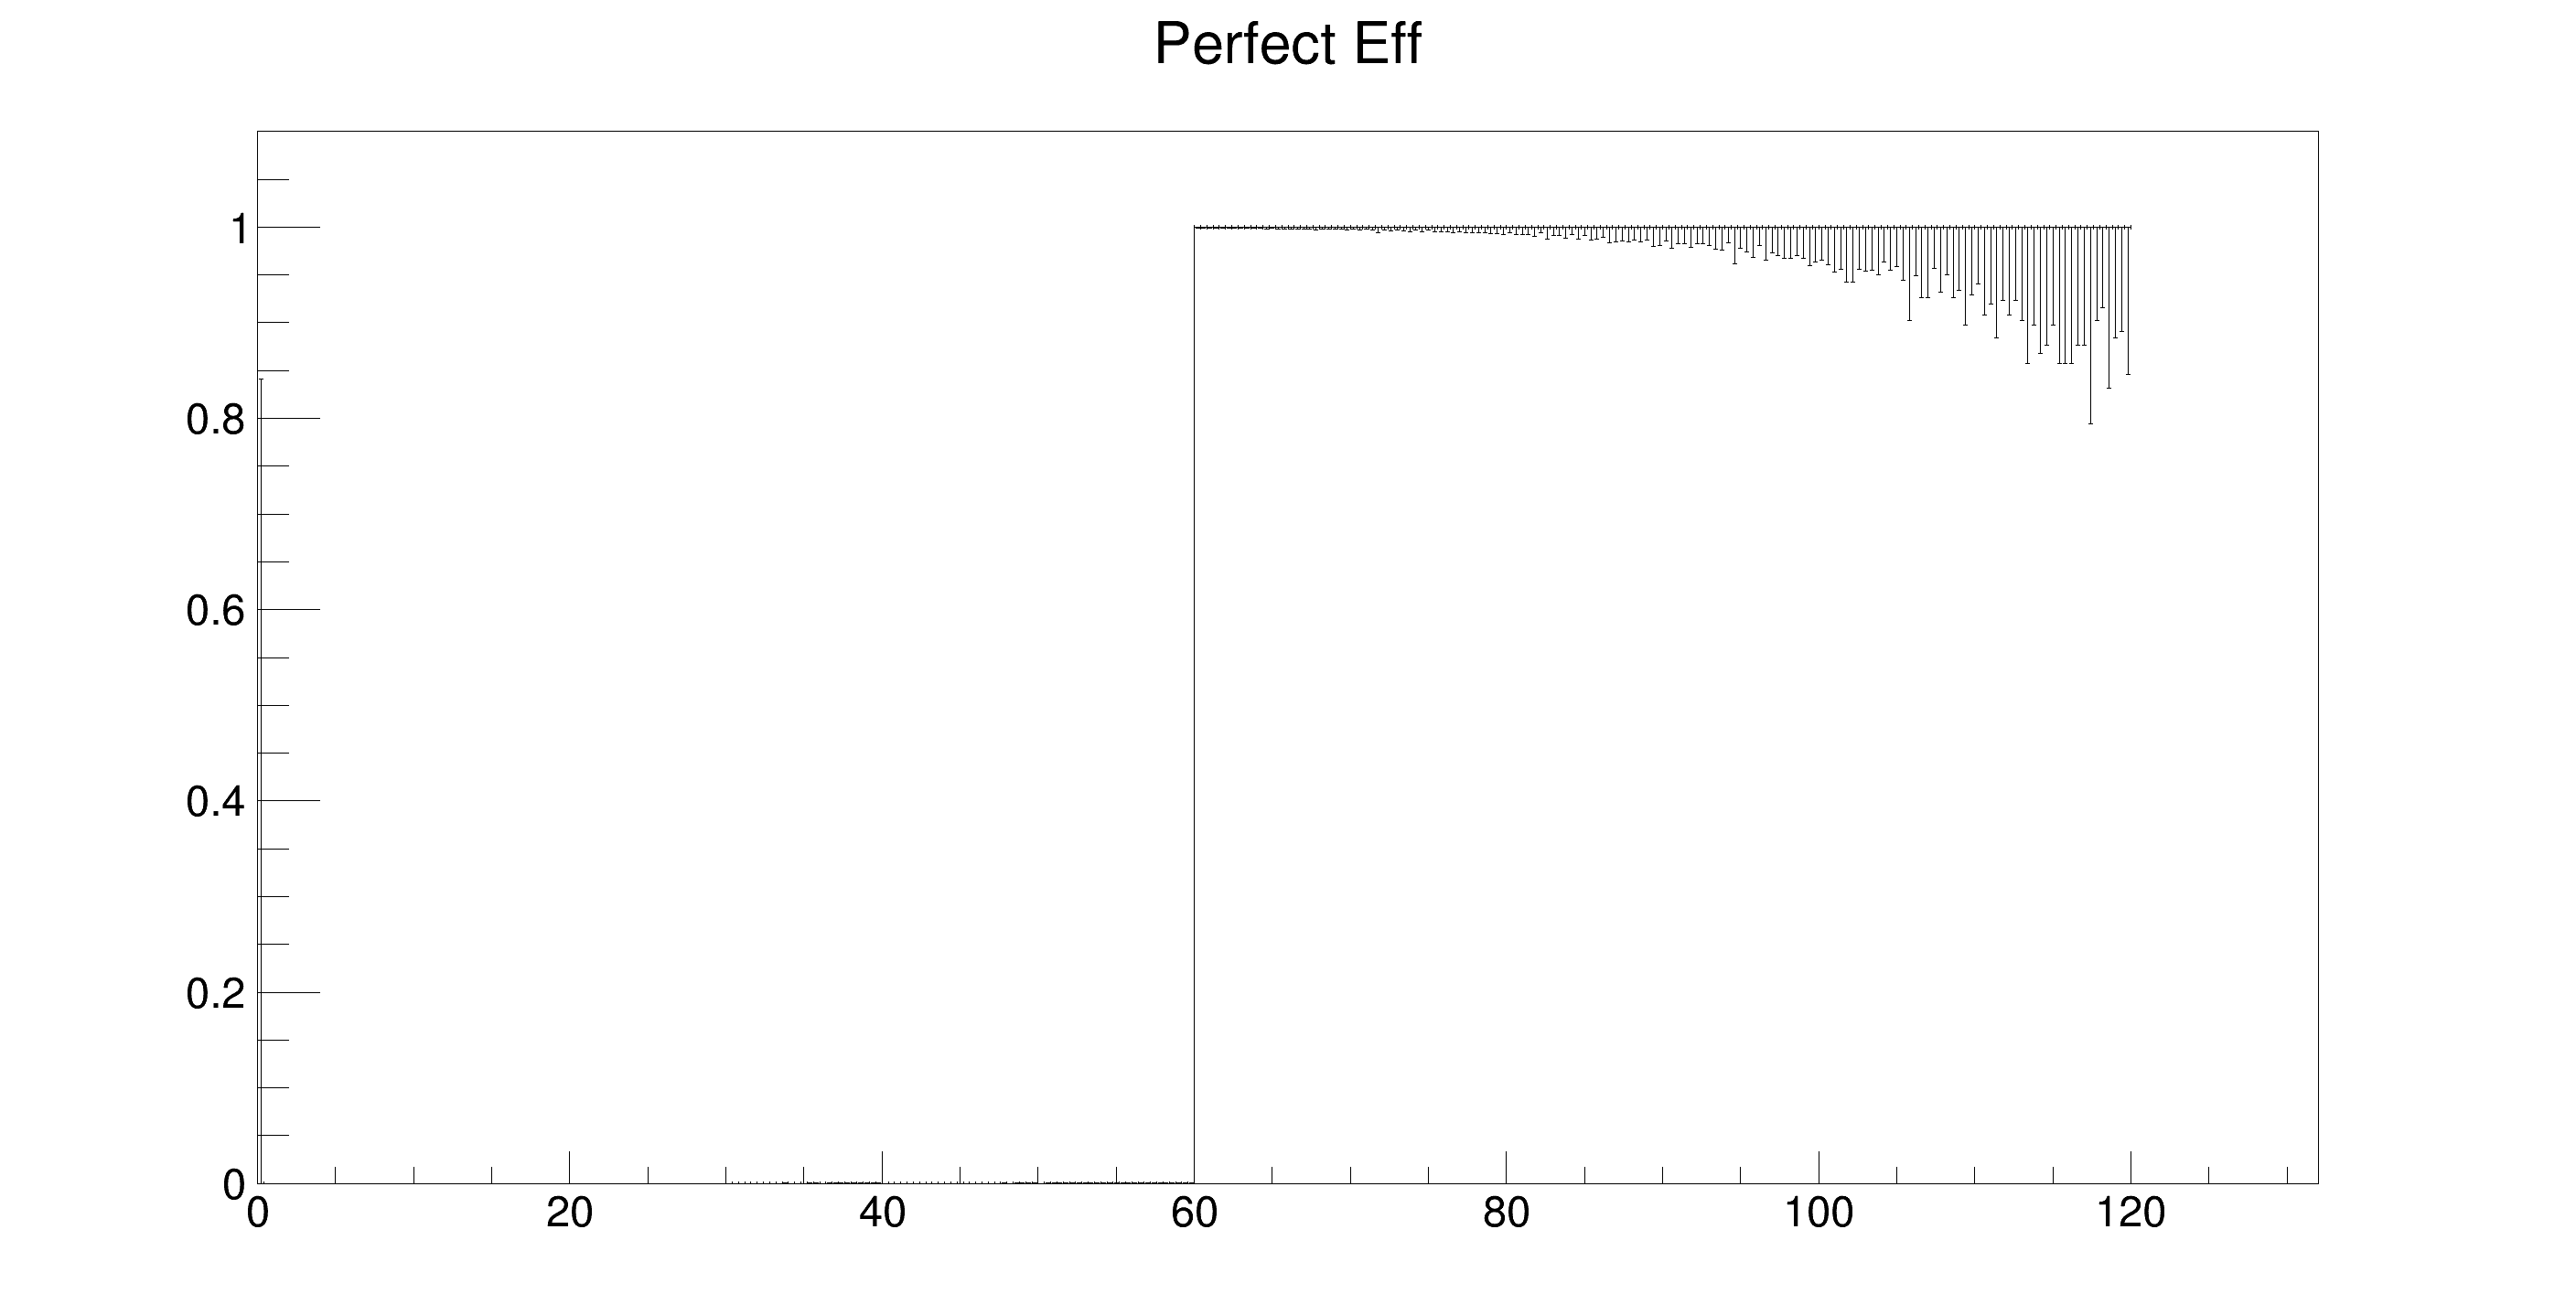
\includegraphics[height=2.65in,width=4.25in]{perfectEfficiency}}
\end{frame}
\begin{frame}{Imperfect Efficiency Curve}
        Here is a plot of the efficiency of $\textrm{L1} > 60.0 \textrm{GeV}$ as a function of CELL MET\\
		\framebox{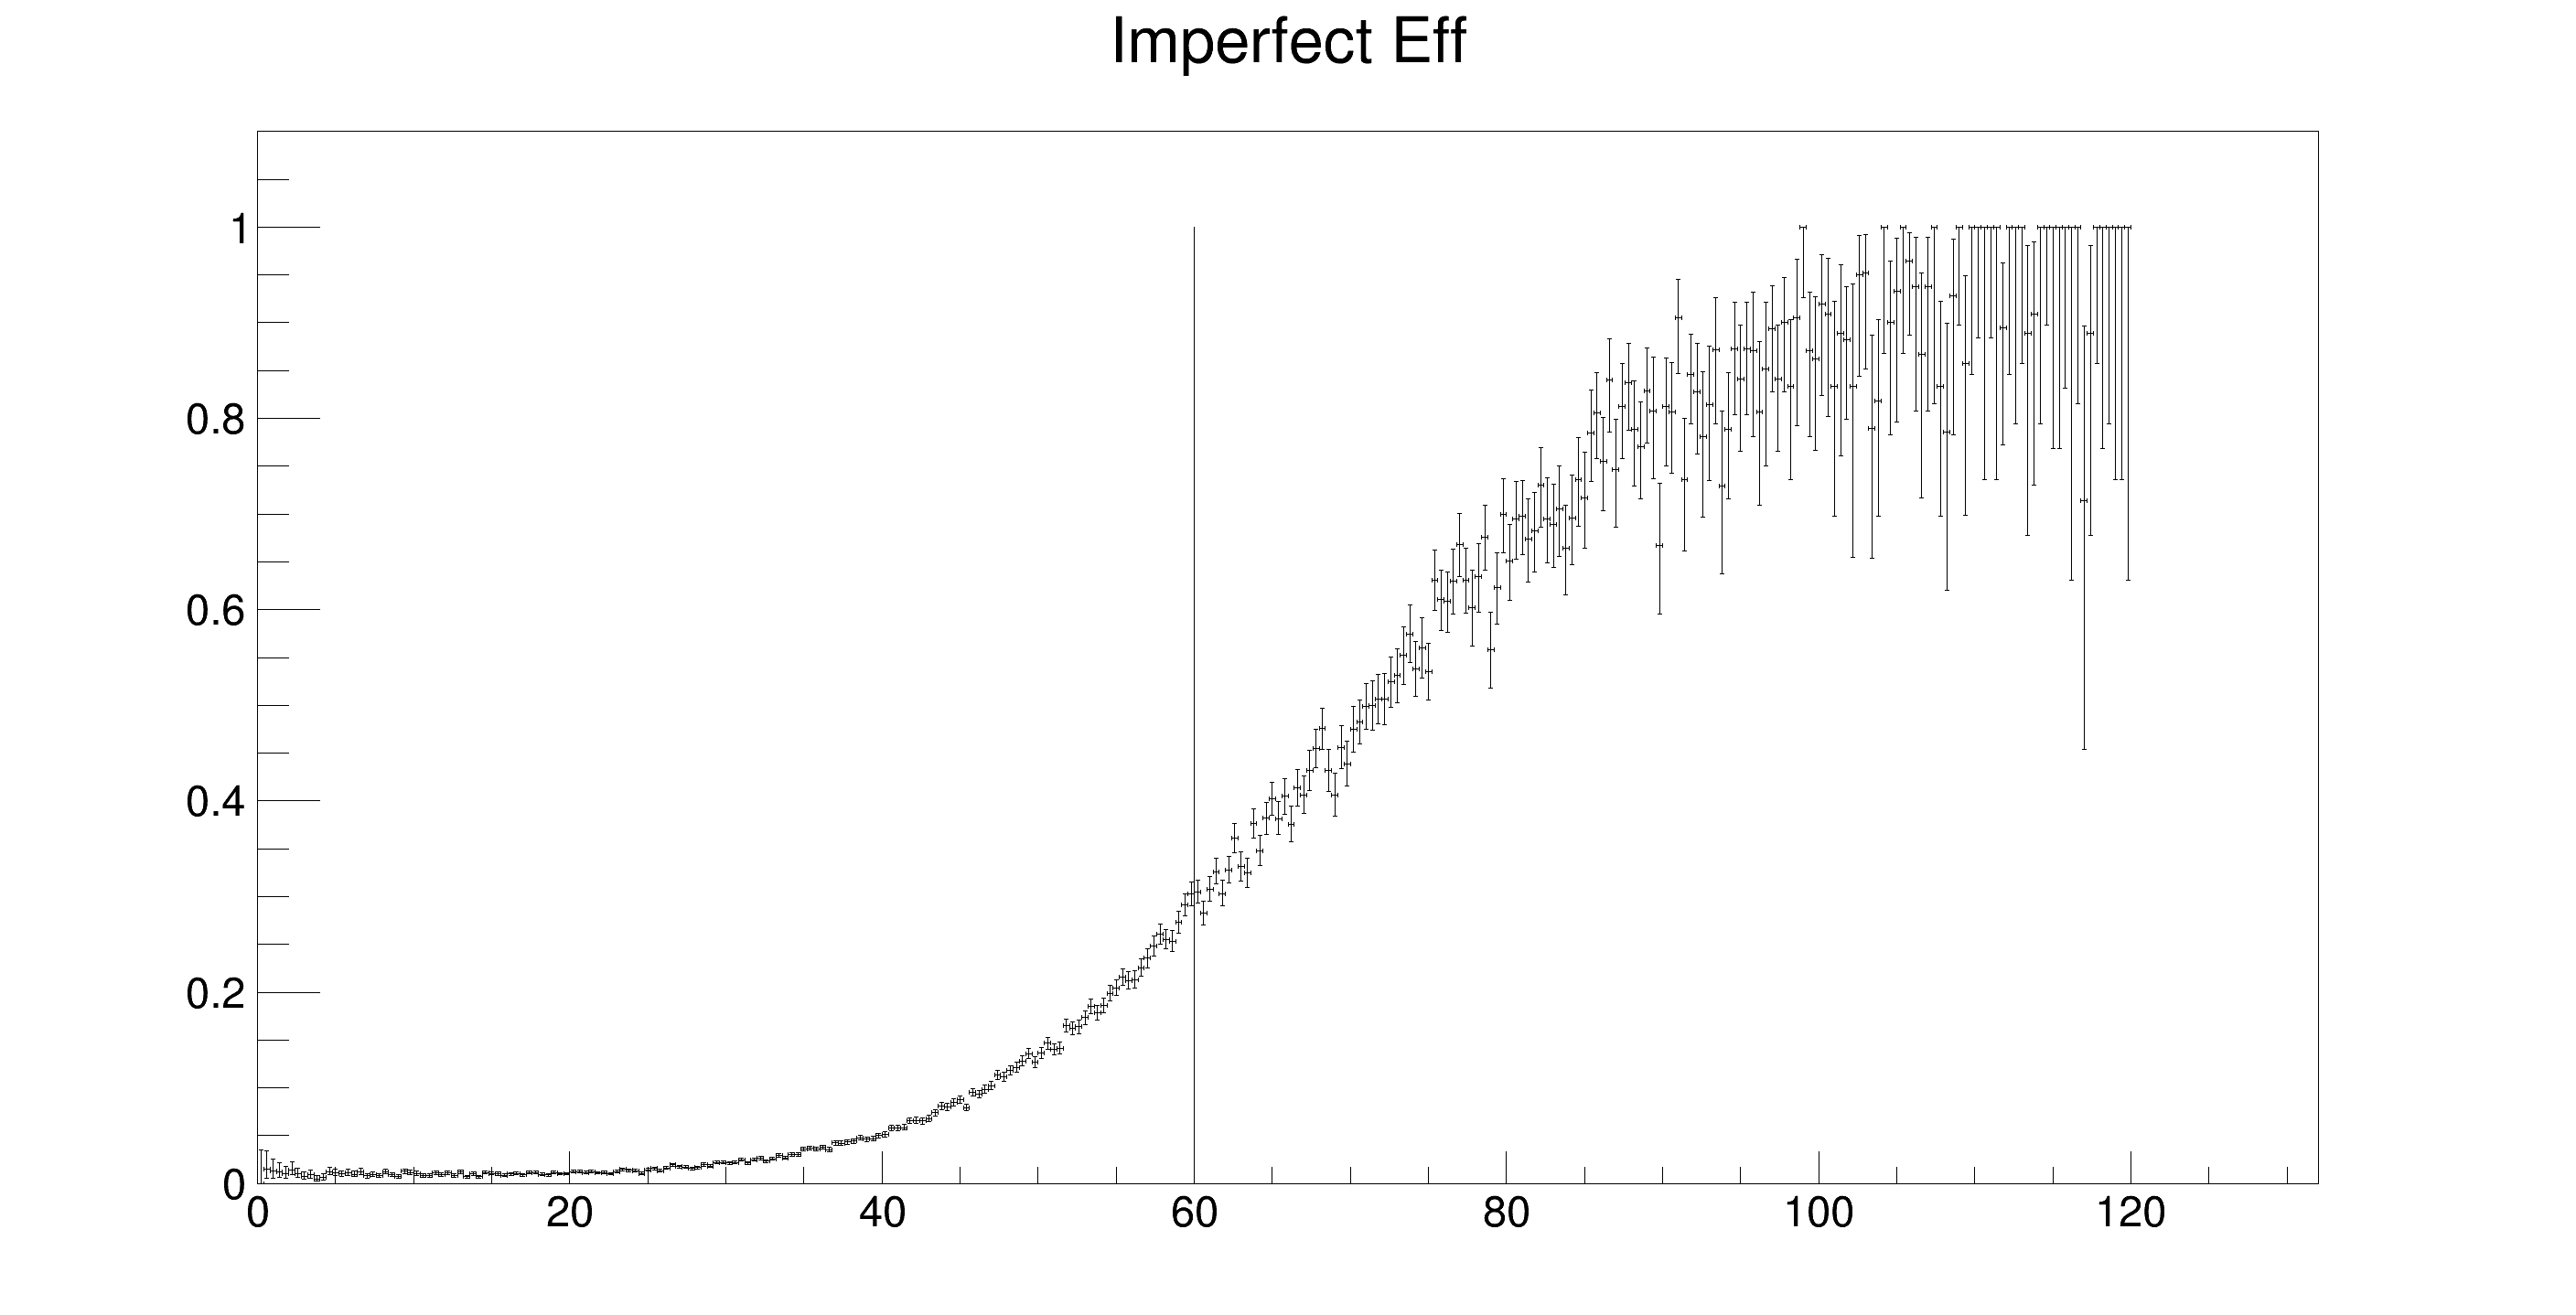
\includegraphics[height=2.65in,width=4.25in]{imperfectEfficiency}}
\end{frame}
\section{Combined Efficiency}
\begin{frame}
\begin{itemize}
        \item We would like to improve the efficiency of event selection by combining algorithms 
        \item Combine two uncorrelated algorithms such that they keep the trigger rate when combined 
		\item The trigger rate is determined by the fraction of background events that are kept by the trigger system
		\item We computed the trigger rate to be the fraction of zerobias events that passed an L1 cut of 50 GeV and a CELL cut of 100 GeV
\end{itemize}
\end{frame}
\begin{frame}{Bisection}
		\begin{itemize}
				\item In order to simplify the problem, we also constrained the algorithms to individually keep the same trigger rate when used alone
				\item After doing this, our problem was essentially one-dimensional and we used a popular root-finding method (bisection) in order to find a solution, subject to the equal fraction constraint, of the equation:
						\begin{align}
								f(\tau_{\alpha},\tau_{\beta})=\textrm{trigger rate}
						\end{align}
		\end{itemize}
\end{frame}
\begin{frame}
		\framebox{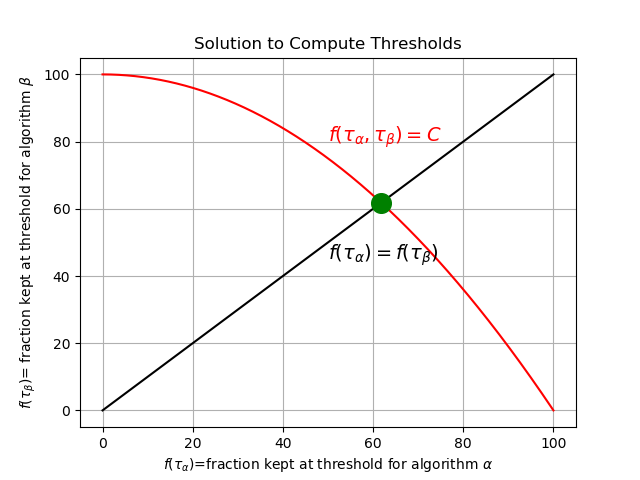
\includegraphics[height=2.65in,width=4.25in]{combined_constraint_plot}}
\end{frame}
\begin{frame}{Combined Efficiency}
		\begin{itemize}
				\item After solving the problem of figuring out what thresholds are needed to keep the trigger rate when the algorithms are used together, we then compute the efficiency of this new algorithm on signal events
				\item The signal events we used are those for which the muon trigger fired, indicating the production of muons
		\end{itemize}
\end{frame}
\section{Results}
\begin{frame}{Results}
        \begin{itemize}
                \item For some pairs of algorithms, we found no increase in overall efficiency by using combined algorithms
                \item However, for other pairs, we did find an increase in efficiency by using the combined algorithms
				\item During the summer of 2018, the pufit and cell combined algorithm trigger was the main trigger that was used for the second part of Run 2.
        \end{itemize}
\end{frame}
\begin{frame}{Algorithms that Don't Do Better Together}
		\framebox{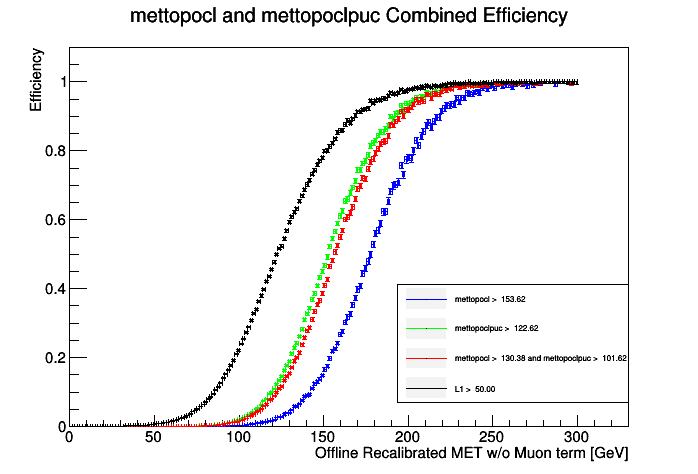
\includegraphics[height=2.65in,width=4.25in]{topocl_puc_efficiencies}}
\end{frame}
\begin{frame}{Algorithms that Do Better Together}
		\framebox{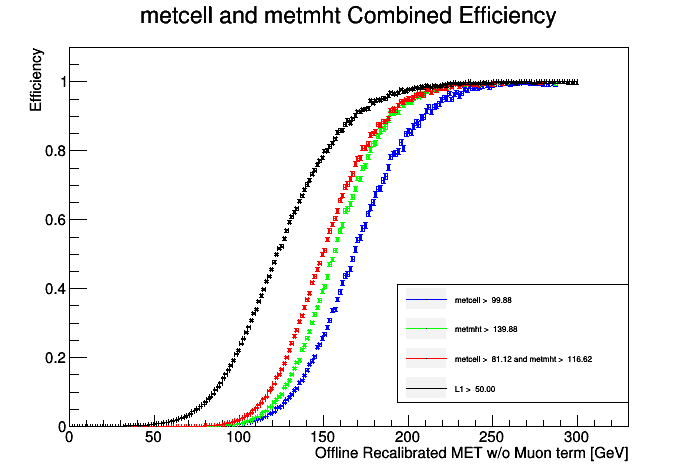
\includegraphics[height=2.65in,width=4.25in]{cell_mht_efficiencies}}
\end{frame}
\begin{frame}
		\framebox{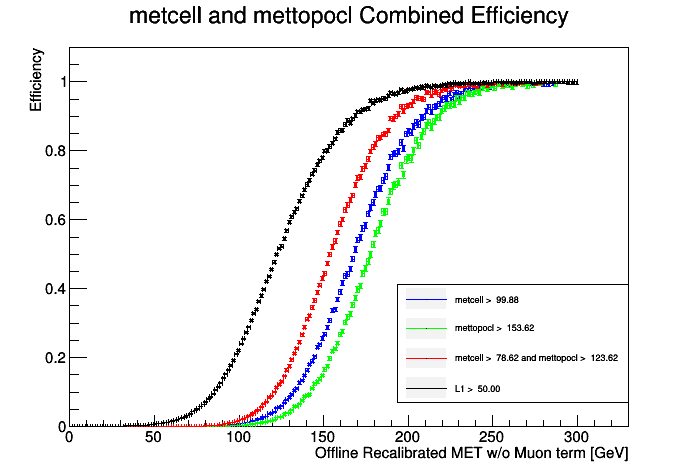
\includegraphics[height=2.65in,width=4.25in]{cell_topocl_efficiencies}}
\end{frame}
\begin{frame}
		\framebox{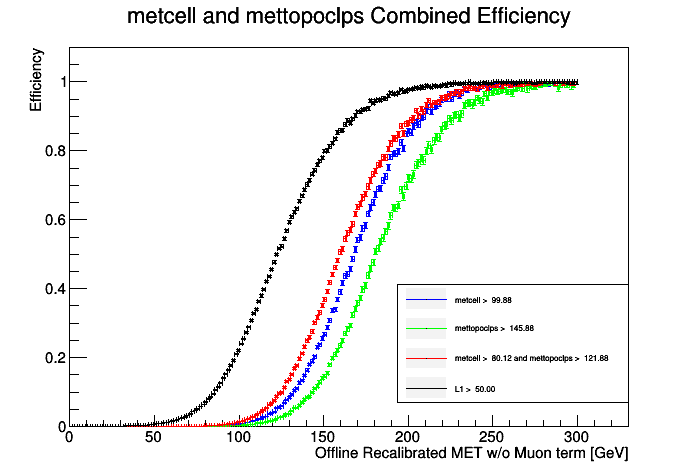
\includegraphics[height=2.65in,width=4.25in]{cell_ps_efficiencies}}
\end{frame}
\begin{frame}
		\framebox{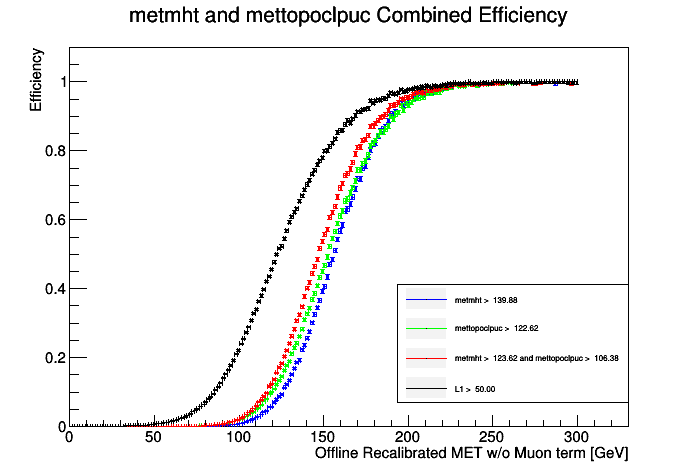
\includegraphics[height=2.65in,width=4.25in]{mht_puc_efficiencies}}
\end{frame}
\begin{frame}{Plot of Best Individual and Best Combined Algorithms}
		\framebox{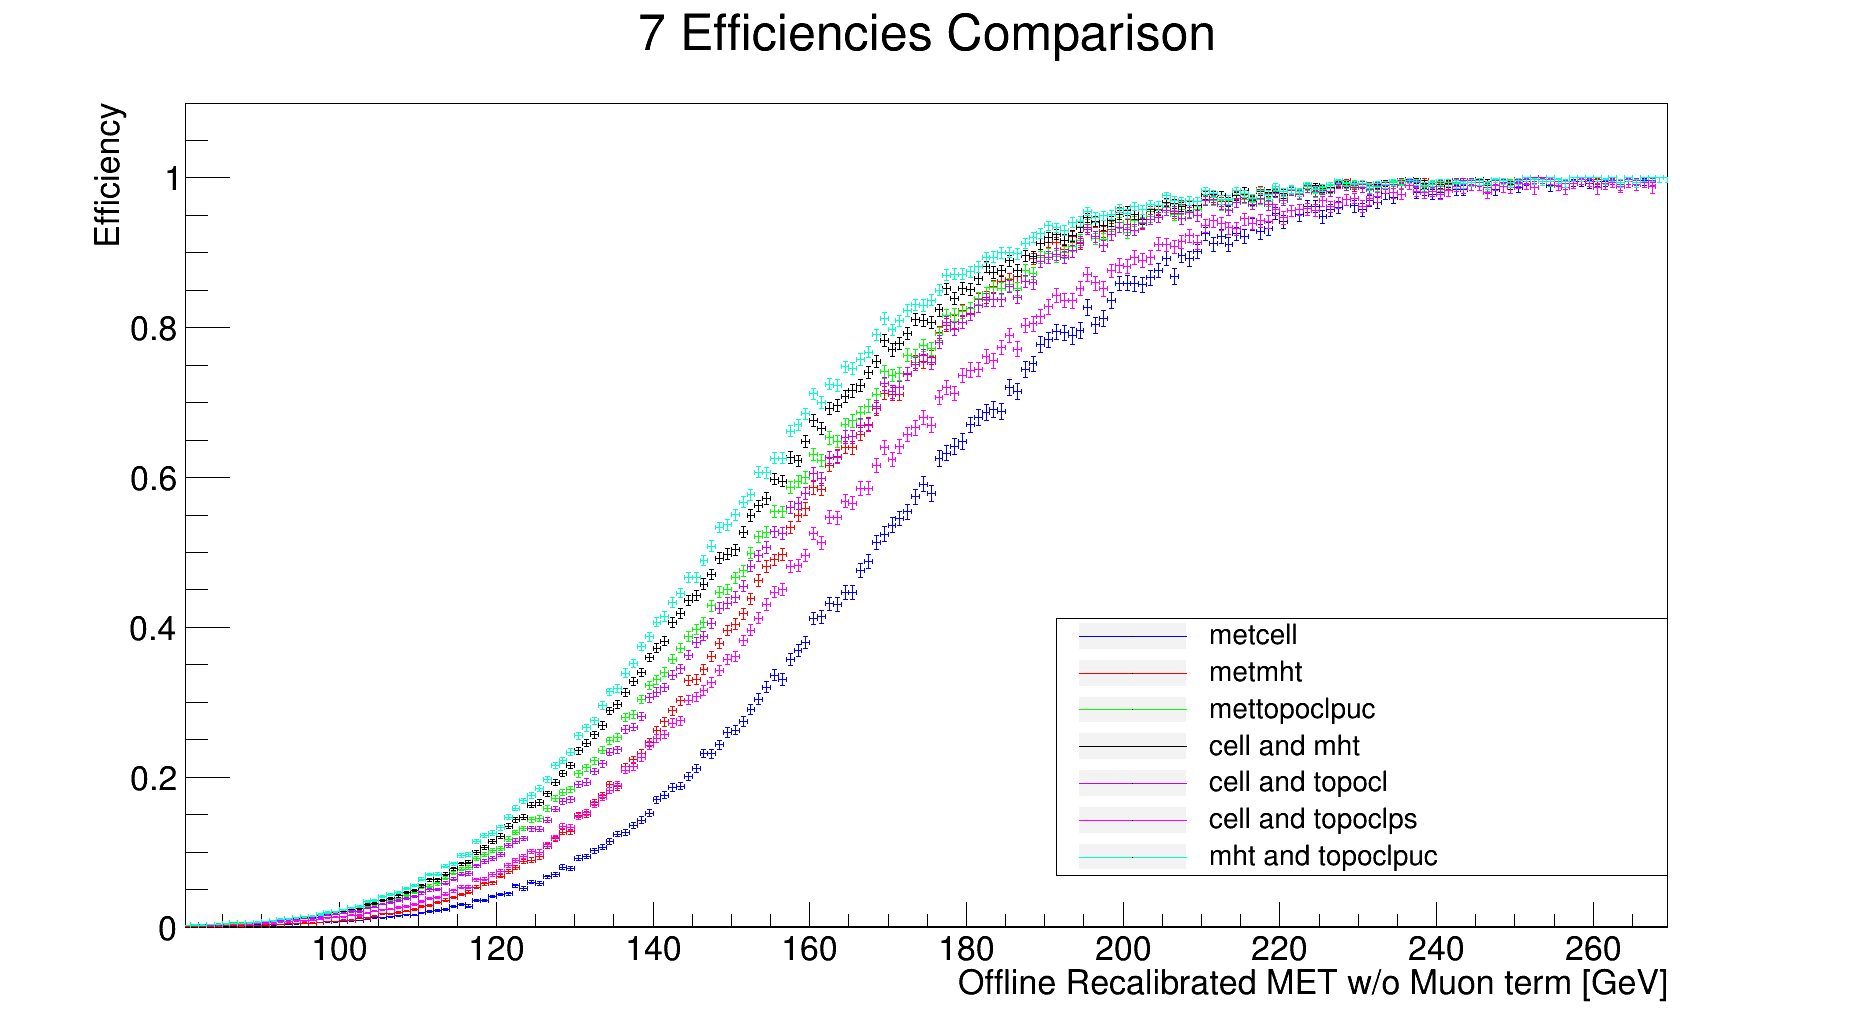
\includegraphics[height=2.65in,width=4.25in]{7Efficiencies}}
\end{frame}
\section{Reconstructing the Unbiased CELL Distribution}
\begin{frame}{Reconstructing the Unbiased CELL Distribution}
\begin{itemize}
        \item Determine CELL MET Distribution as a function of $\mu$
        \item Zerobias events run out of statistics above about 80 GeV
        \item Use \texttt{HLTnoalg\_L1XExx} triggered events to extend to higher MET.
        \item Correct the HLTnoalg Data Using Efficiency determined from lower threshold triggers.
        \item Determine errors including statistical and those due to determination of efficiency.
\end{itemize}
\end{frame}
\section{Method}
\begin{frame}{Method}
For each bin of actual number of interactions per bunch crossing (actint/InTimePileup):
\begin{enumerate}
        \item Compute the Efficiency of L1XE 30 for \texttt{HLTzb\_L1ZB} events as a function of cell met
        \item Obtain an unbiased (with respect to L1) CELL MET distribution from the \texttt{HLTnoalg\_L1XE30} data by multiplying by the prescale and dividing by efficiency computed previously
        \item Compute efficiency of L1XE50 for \texttt{HLTnoalg\_L1XE30} data as a function of cell met
        \item Obtain an unbiased (with respect to L1) CELL MET distribution from the \texttt{HLTnoalg\_L1XE50} data by multiplying by the prescale and dividing by both of the previously computed efficiencies.
\end{enumerate}
\end{frame}
\begin{frame}{Data Used}
  \begin{itemize}
          \item Used 2015, 2016 and 2017 combined \texttt{HLTnoalg\_L1ZB}, \texttt{HLTnoalg\_L1XE30}, and \texttt{HLTnoalg\_L1XE50} data produced by Jonathan Burr dated 2017-11-17 from ZB and JETM10 trees
		  \item Removed events from Runs 330203, 331975 and 334487. These had large MET events without jets and logbook says there were calorimeter noise problems in these runs
  \end{itemize}
\end{frame}
\section{Efficiency Fits}
\begin{frame}{Efficiency Fits}
		\begin{itemize}
				\item Assume the distribution of L1 MET, given the value of CELL MET, is gaussian. 
				\item Fitted an error function to the efficiency to evaluate a continuous function when correcting the distribution of \texttt{HLTnoalg} data.
				\item Fit function we used has 4 parameters: $a$, $b$, $\sigma$, and L1XE.
				\item $f(x)=\frac{1}{2}\left( 1+\mathrm{Erf}\left( \frac{ax+b-\mathrm{L1XE}}{\sigma \sqrt{2}} \right) \right)$.
				\item Fit in actint bins of $0-10,\ldots, 60-70$.
		\end{itemize}
\end{frame}
% PLOTS OF ALL EFFICIENCIES AND FITS TOGETHER
\begin{frame}
		\framebox{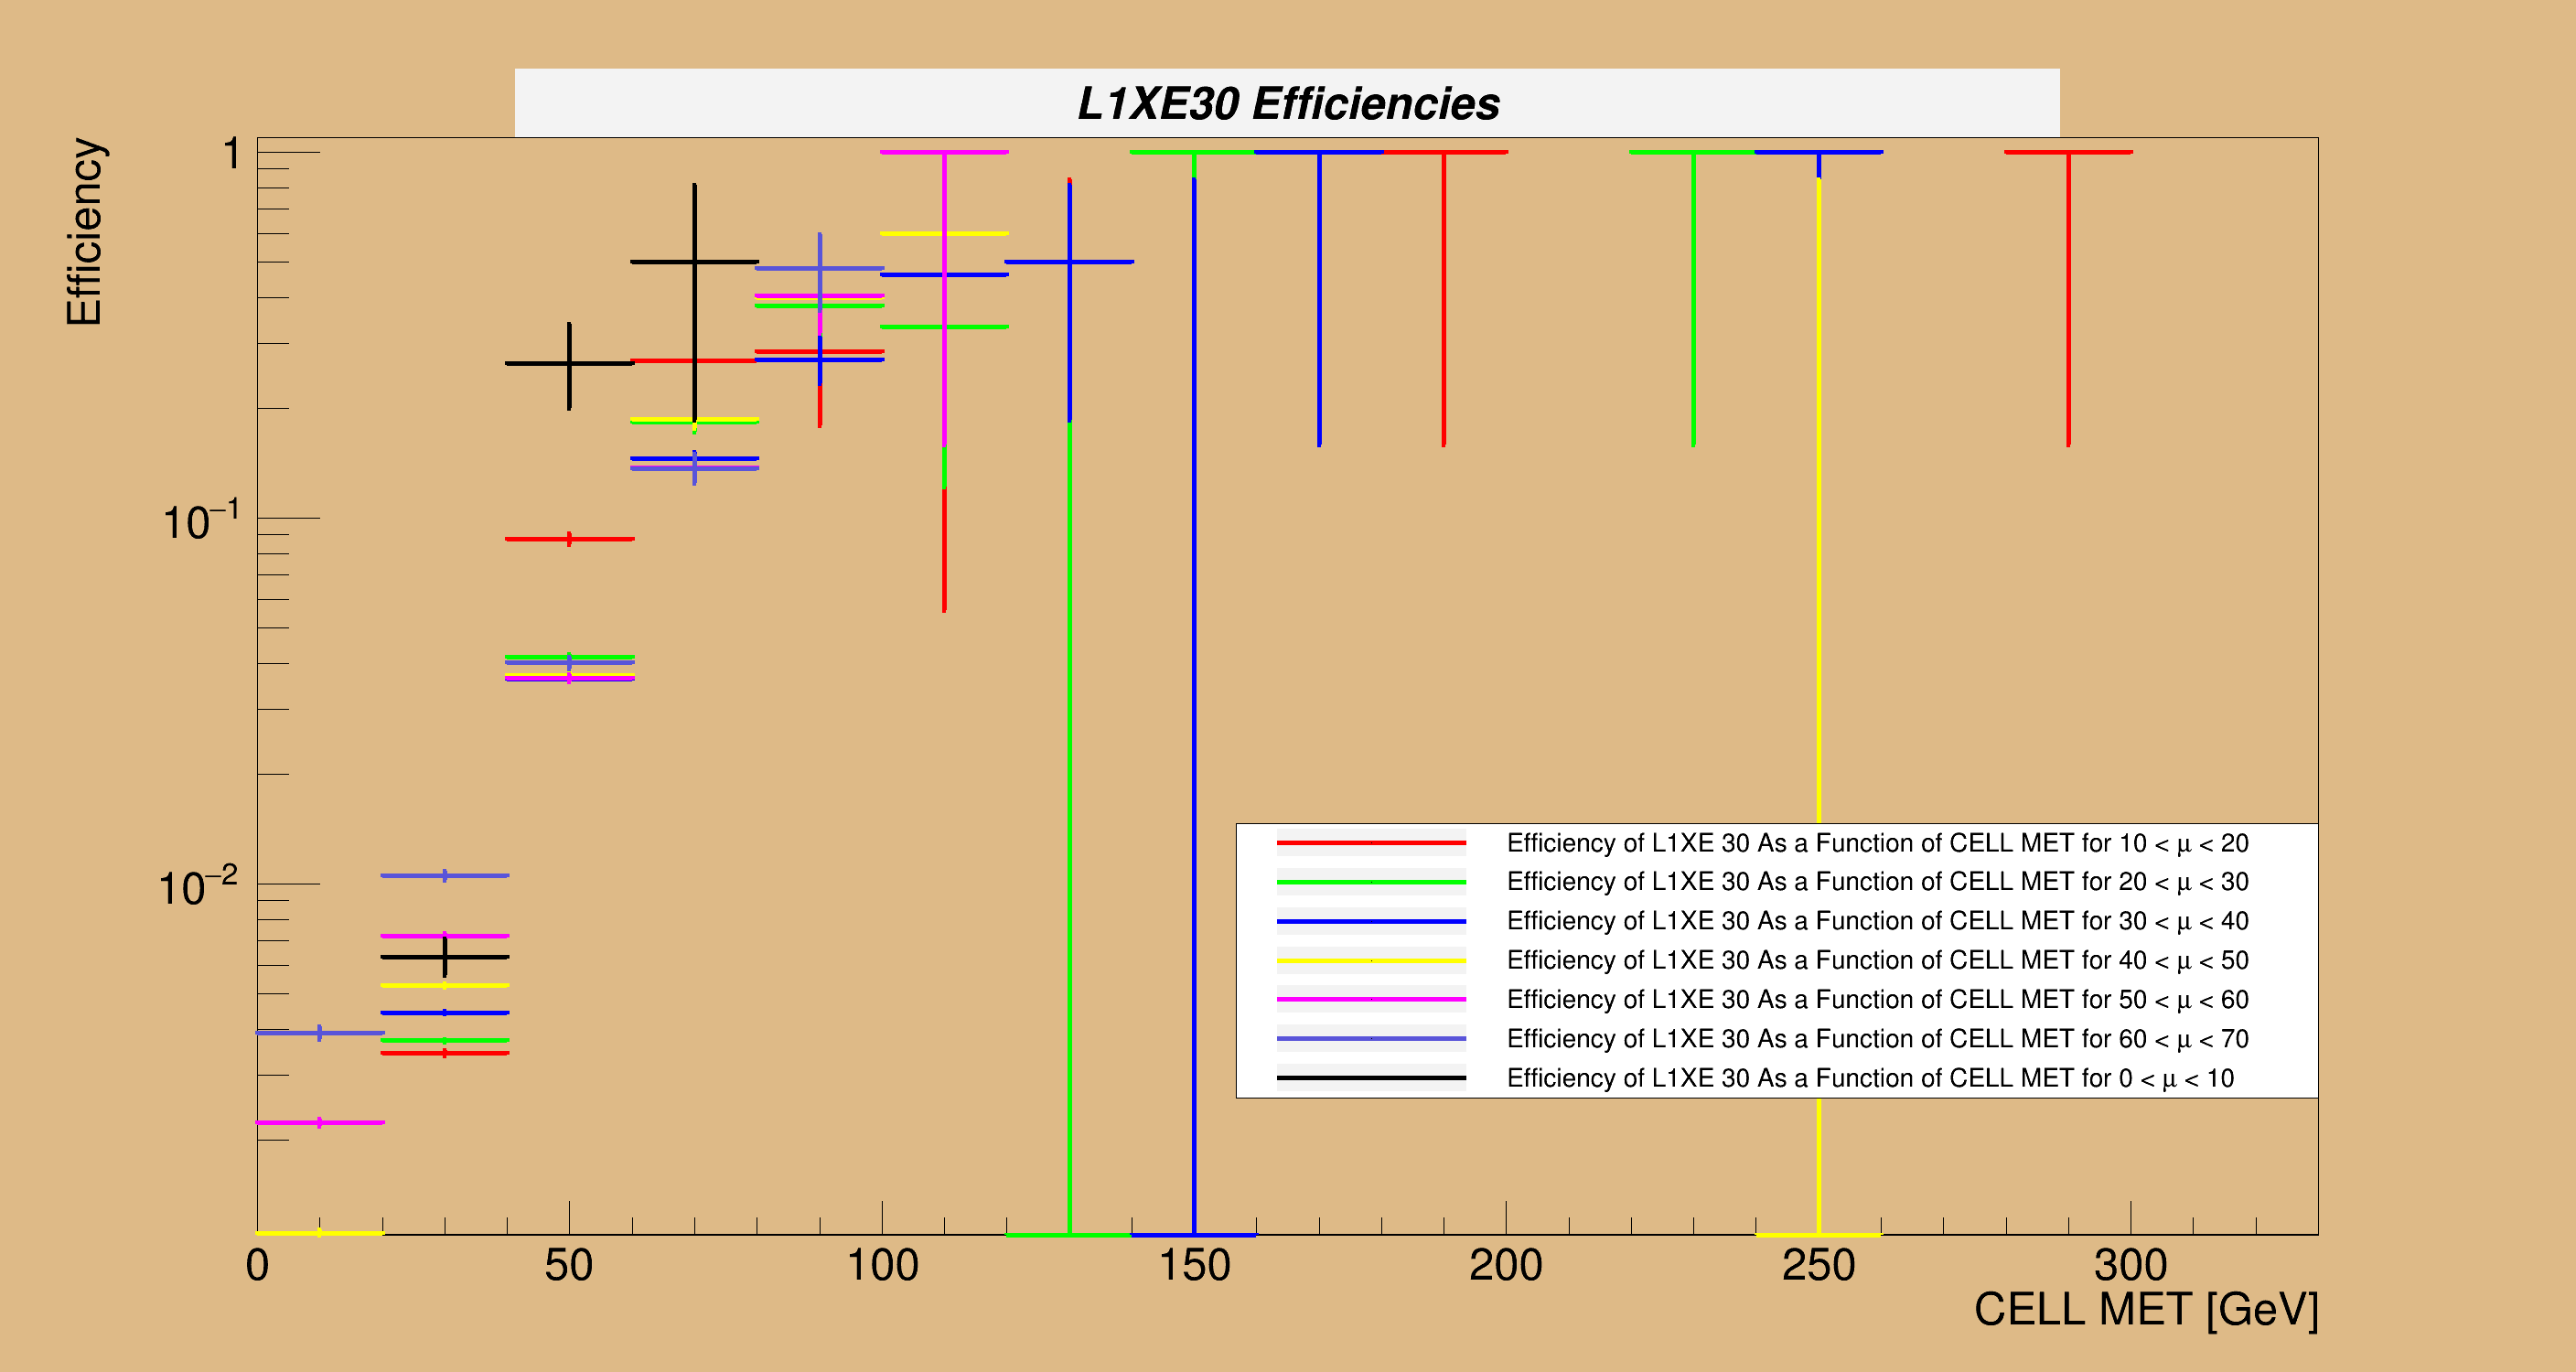
\includegraphics[height=2.65in,width=4.25in]{L1XE30Efficiency_Curves}}
\end{frame}
\begin{frame}
		\framebox{\includegraphics[height=2.65in,width=4.25in]{l1xe30_efficiencies/L1XE30Efficiency_mu_between_30_40}}
\end{frame}
\begin{frame}
		\framebox{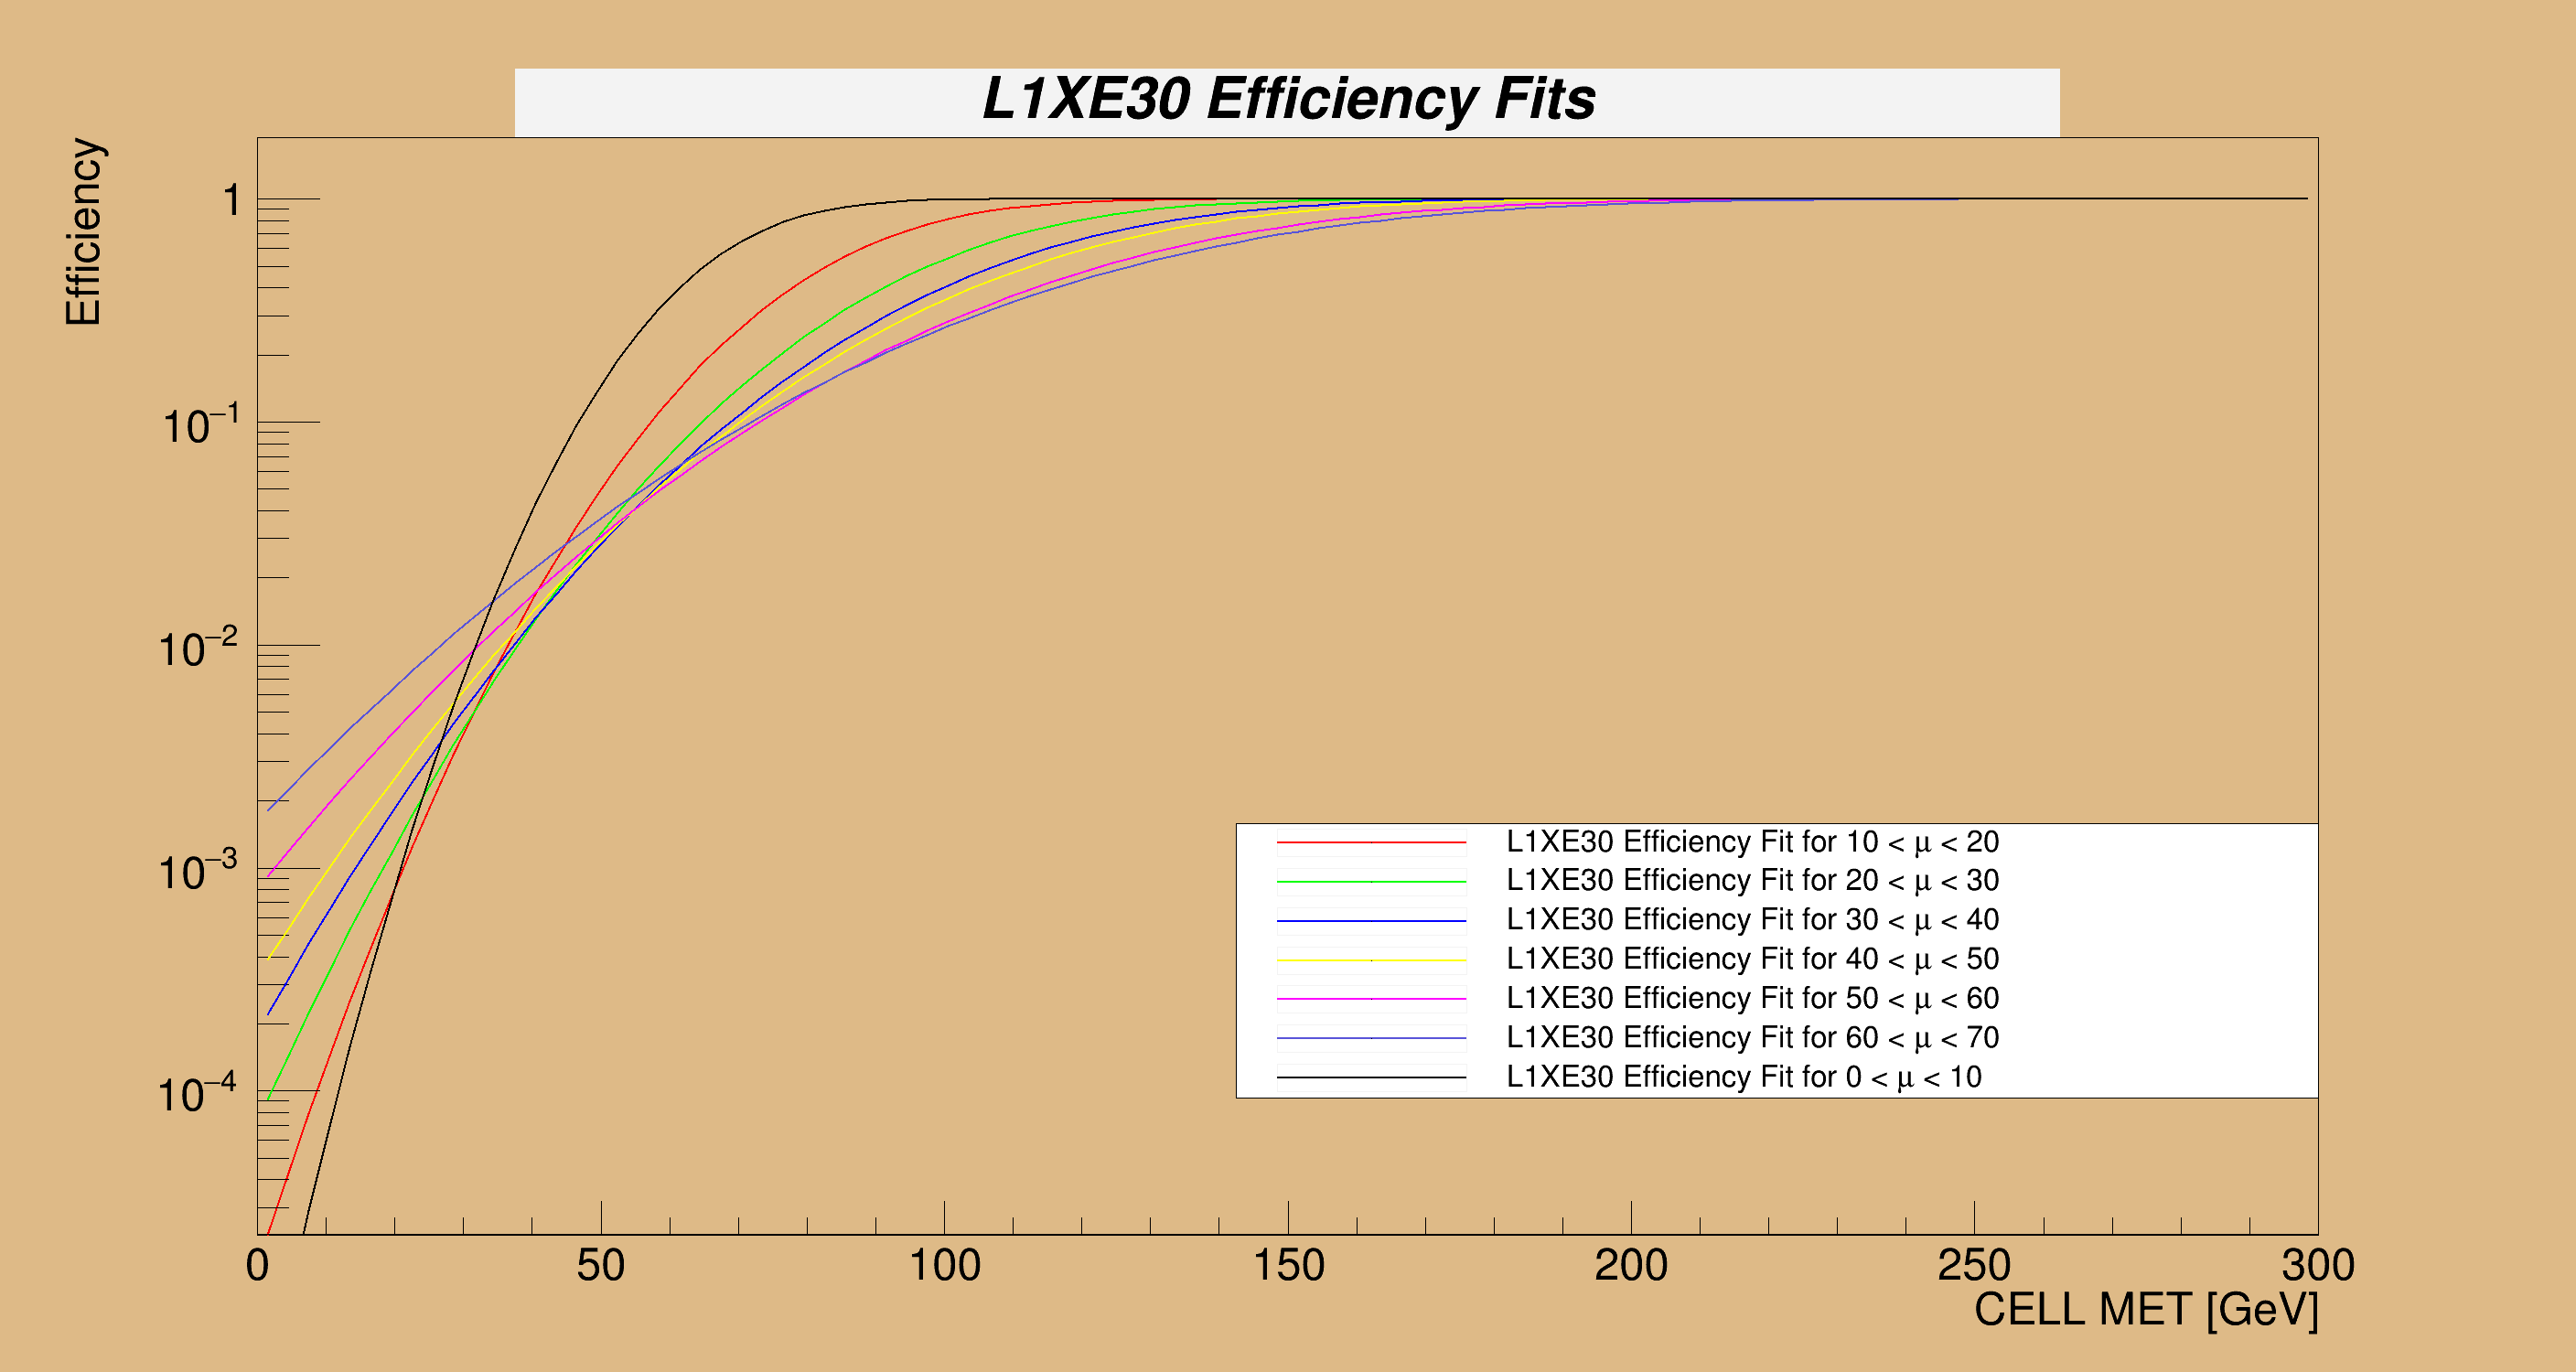
\includegraphics[height=2.65in,width=4.25in]{L1XE30Efficiency_Fits}}
\end{frame}
\begin{frame}
		\framebox{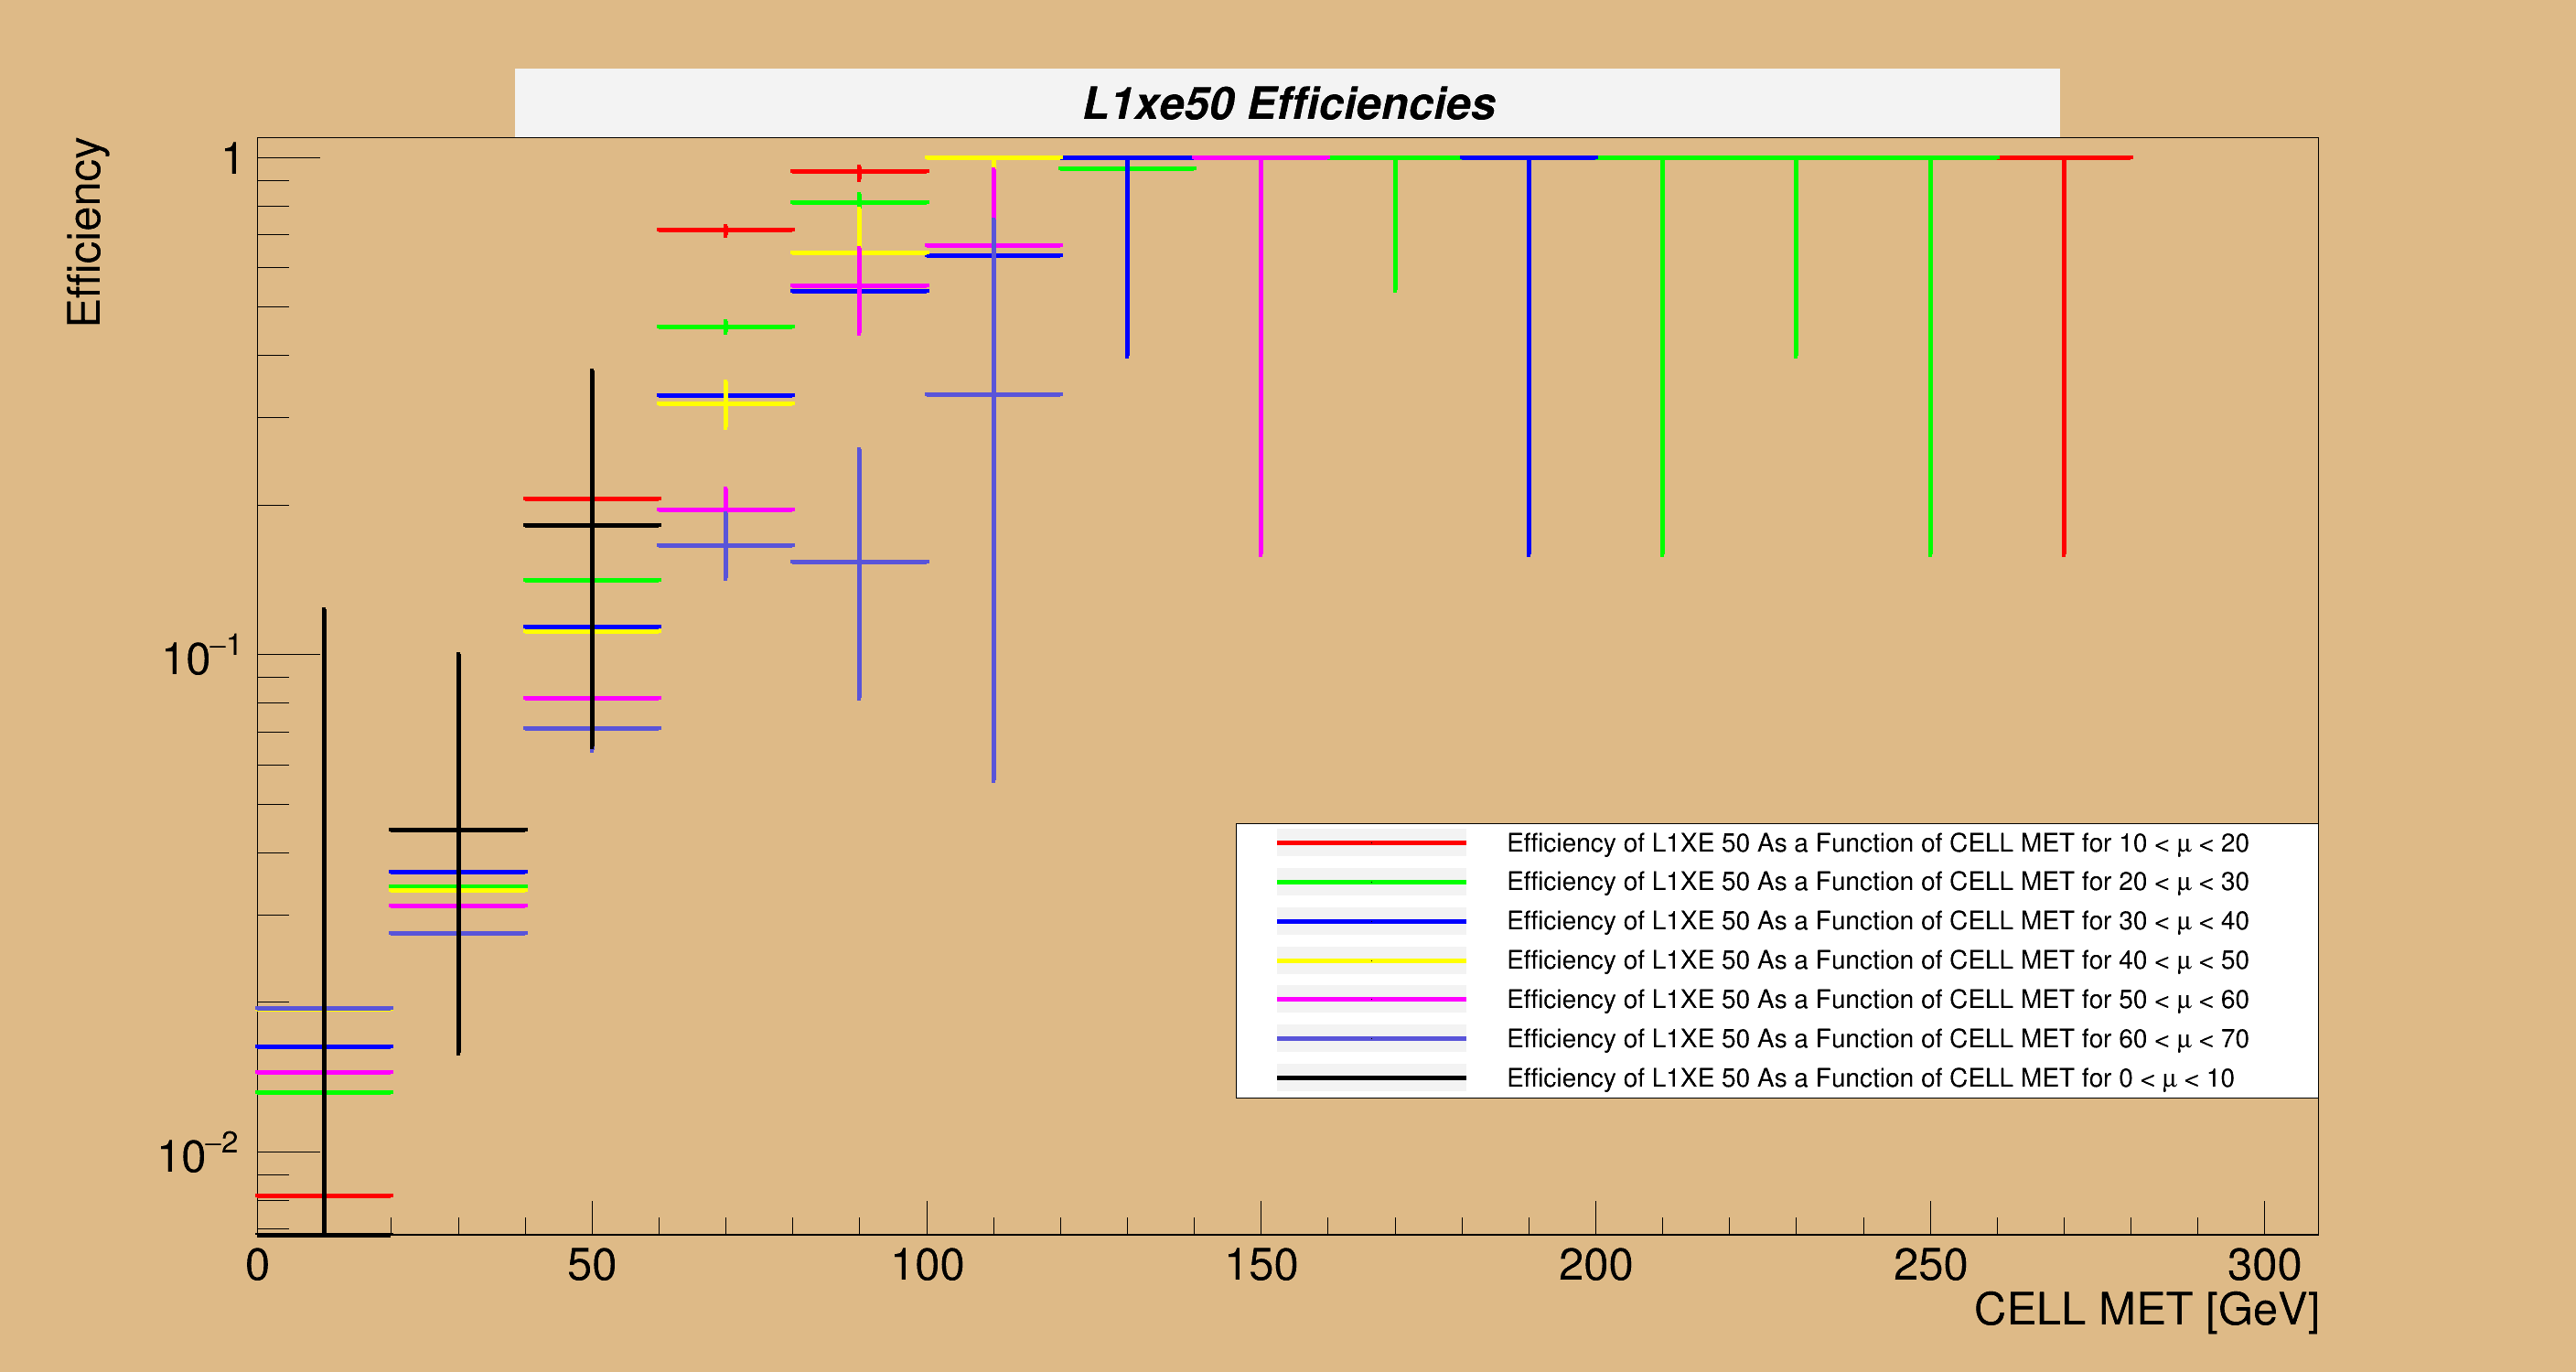
\includegraphics[height=2.65in,width=4.25in]{L1XE50Efficiency_Curves}}
\end{frame}
\begin{frame}
		\framebox{\includegraphics[height=2.65in,width=4.25in]{l1xe50_efficiencies/L1XE50Efficiency_mu_between_30_40}}
\end{frame}
\begin{frame}
		\framebox{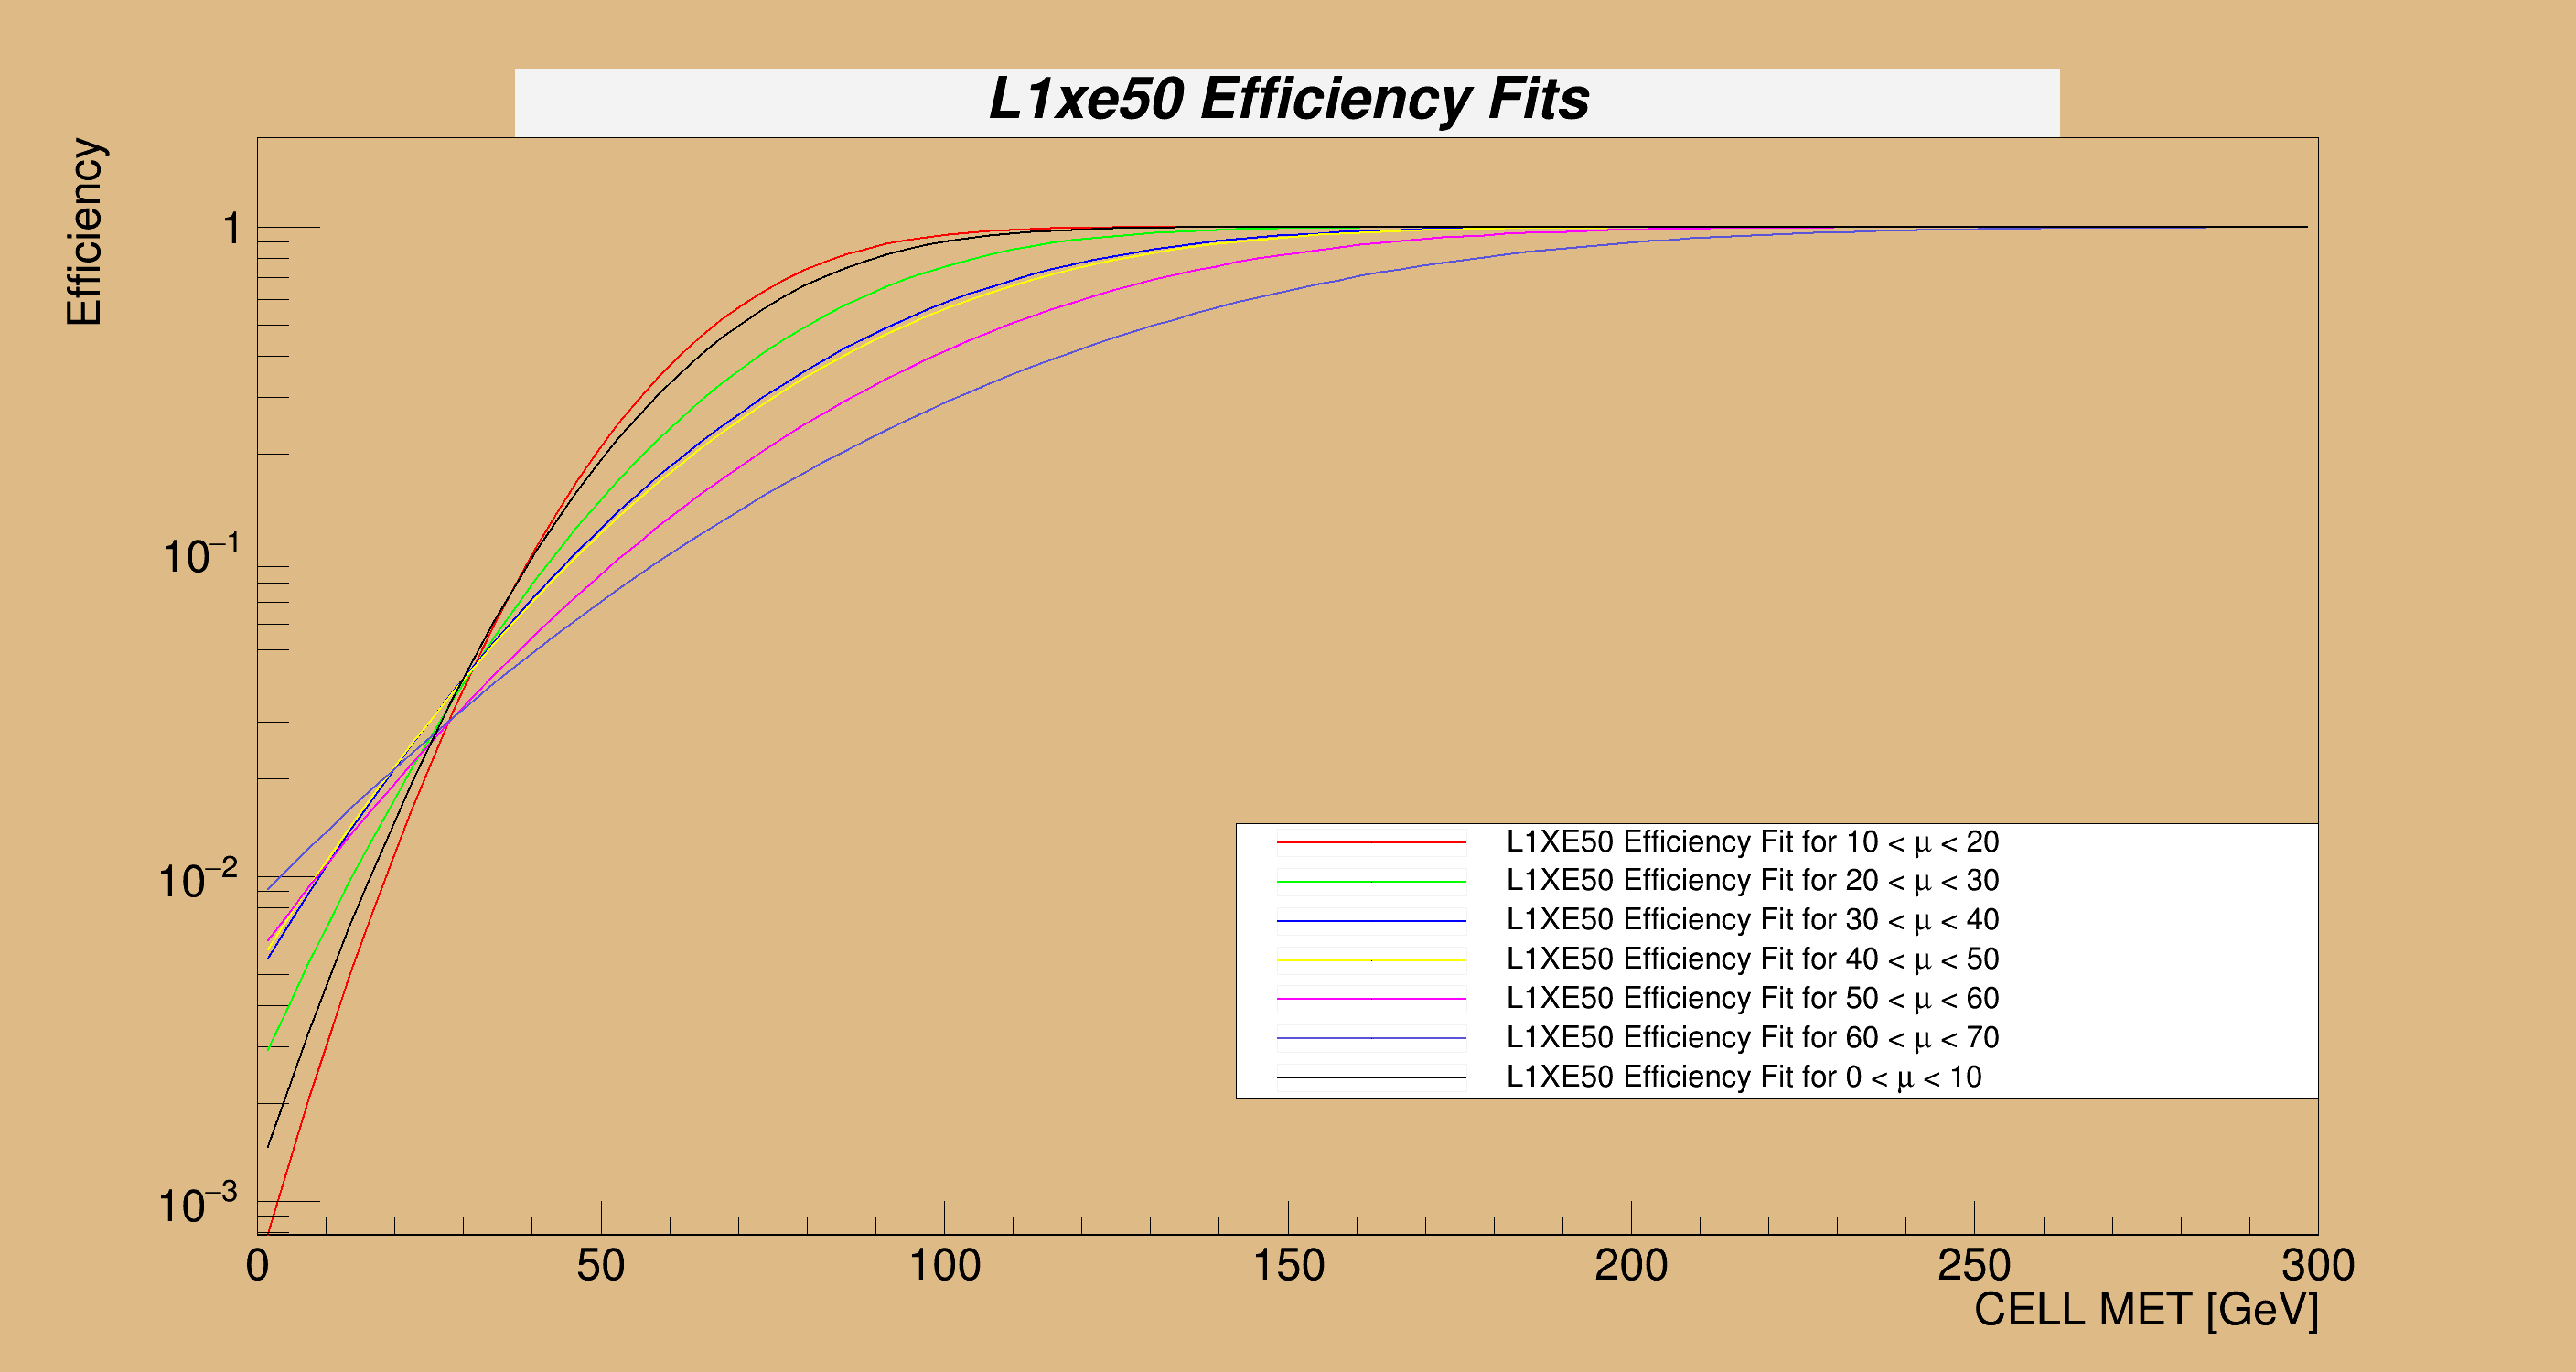
\includegraphics[height=2.65in,width=4.25in]{L1XE50Efficiency_Fits}}
\end{frame}
\section{Performing Correction}
\begin{frame}{Correcting the \texttt{HLTnoalg} Distribution}
		\begin{itemize}
				\item After computing the efficiency curves for the cuts on L1, the curves were used to correct the HLTnoalg distributions that are biased with respect to L1 so that they replicate the unbiased distribution
				\item In order to do this, it was necessary to multiply by the recorded prescale, and divide by the efficiency used to correct the data
				\begin{itemize}
						\item For the \texttt{HLTnoalg\_L1XE30} data, we used the \texttt{L1XE30} efficiency curve to correct the distribution
						\item For the \texttt{HLTnoalg\_L1XE50} data we used the \texttt{L1XE30} efficiency of the zerobias data, as well as the L1XE50 efficiency of \texttt{HLTnoalg\_L1XE30} data to correct the distribution
				\end{itemize}
		\end{itemize}
\end{frame}
\section{Error Propagation}
\begin{frame}{Error Propagation}
		\begin{itemize}
				\item The error in each efficiency value is determined by propagating the errors on the parameters of the respective fit function.
				\item The reconstructed MET distribution includes both the error determined above, and the statistical error. 
				\item Since prescales vary for each bin, must keep track of errors event by event, rather than using ROOT’s built-in errors. 
				\item Kept track of the errors on the \texttt{L1XE30} corrected curves, as well as the \texttt{L1XE50} corrected curves, for each of the mu bins
                \item There is no error included to reflect the fact that the error function may not be a perfect model. Therefore, in final distribution, zerobias data is kept to as high an MET as possible and similarly for keeping \texttt{HLTnoalg\_L1XE30} versus \texttt{HLTnoalg\_L1XE50}
        \end{itemize}
\end{frame}
\begin{frame}
		\framebox{\includegraphics[height=2.65in,width=4.25in]{hlt_noalg_l1xe30_plots/hlt_noalg_L1XE30_dist_mubin_3}}
\end{frame}
\begin{frame}
		\framebox{\includegraphics[height=2.65in,width=4.25in]{hlt_noalg_l1xe50_plots/hlt_noalg_L1XE50_dist_mubin_3}}
\end{frame}
\begin{frame}{Relative Normalization}
		\begin{itemize}
				\item Because the error bars are larger at low values of MET, it is not sufficient to normalize the entire curve to one. Instead, it was necessary to perform a relative overall normalization between the original zerobias distribution and the corrected curves in order to be able to compare the shapes more easily.
				\item The relative normalization factor was computed by taking a weighted average of ratios computed in the region where the slopes look most parallel.
                \item The following slides show all 3 sets of data points after all corrections and the relative normalization (from the corrected HLTnoalg data to the unbiased distribution) have been done.
                \item The vertical black lines on the bottom efficiency curve plots show where I've stopped using the zerobias data and started using the \texttt{HLTnoalg\_L1XE30} and \texttt{HLTnoalg\_L1XE50} data, respectively.
		\end{itemize}
\end{frame}
\section{Reconstructed Distributions}
\begin{frame}
		\framebox{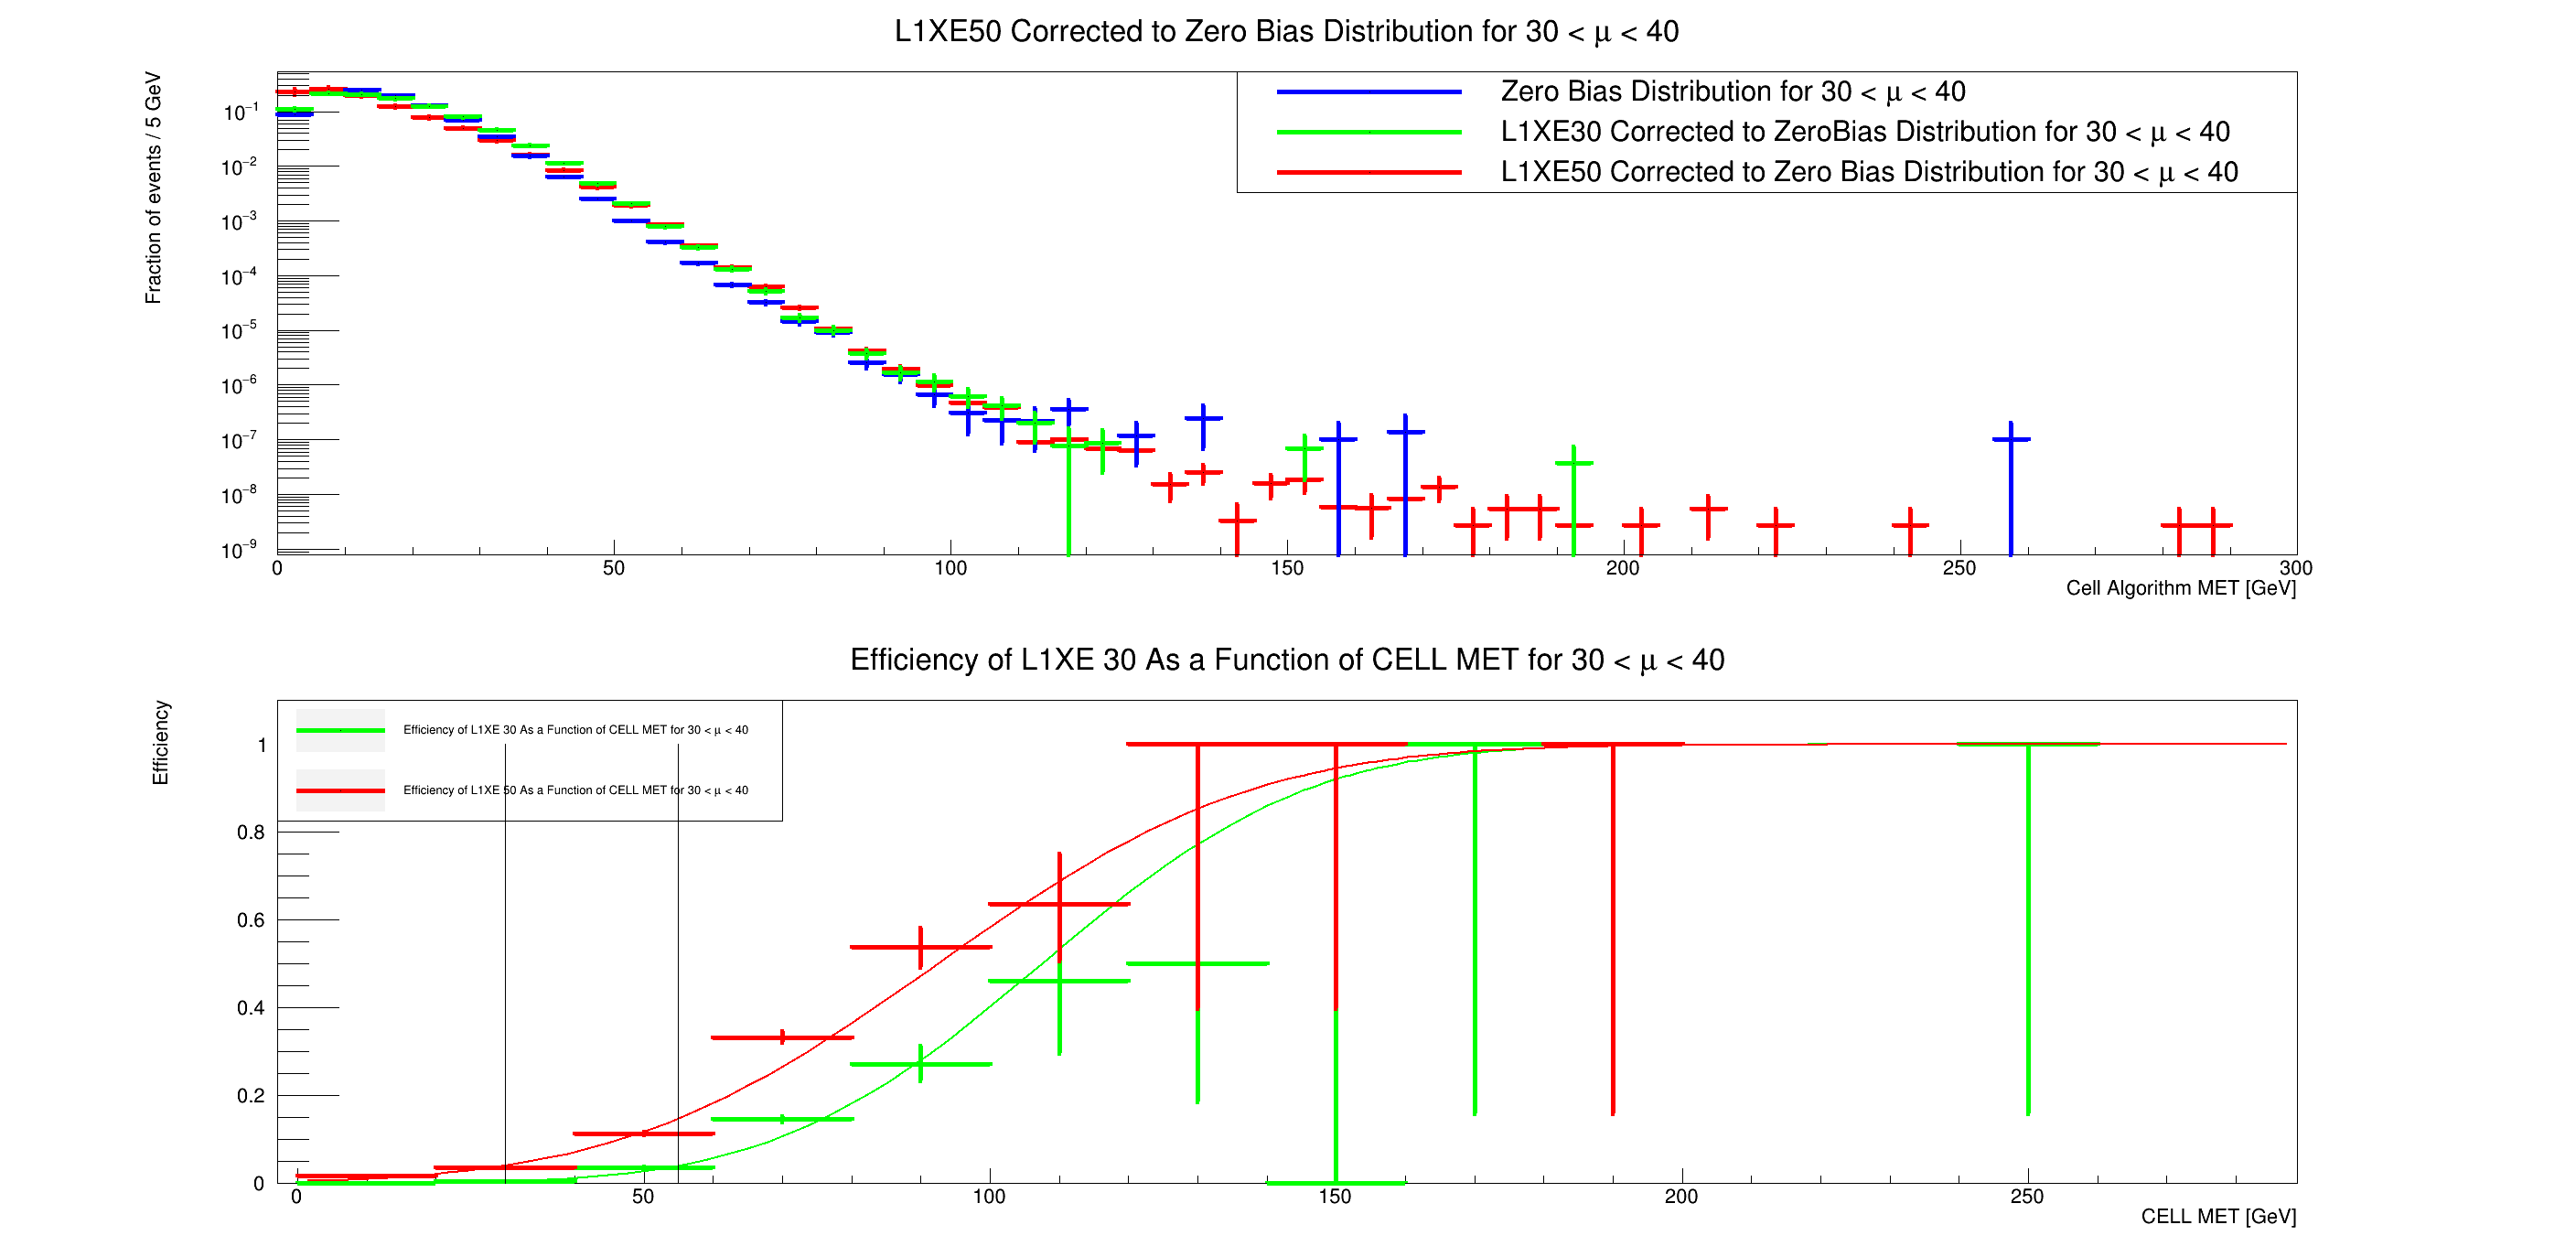
\includegraphics[height=2.65in,width=4.25in]{zerobias_distributions_corrected/zb_met_distributions_mubin_3}}
\end{frame}

\begin{frame}
		\framebox{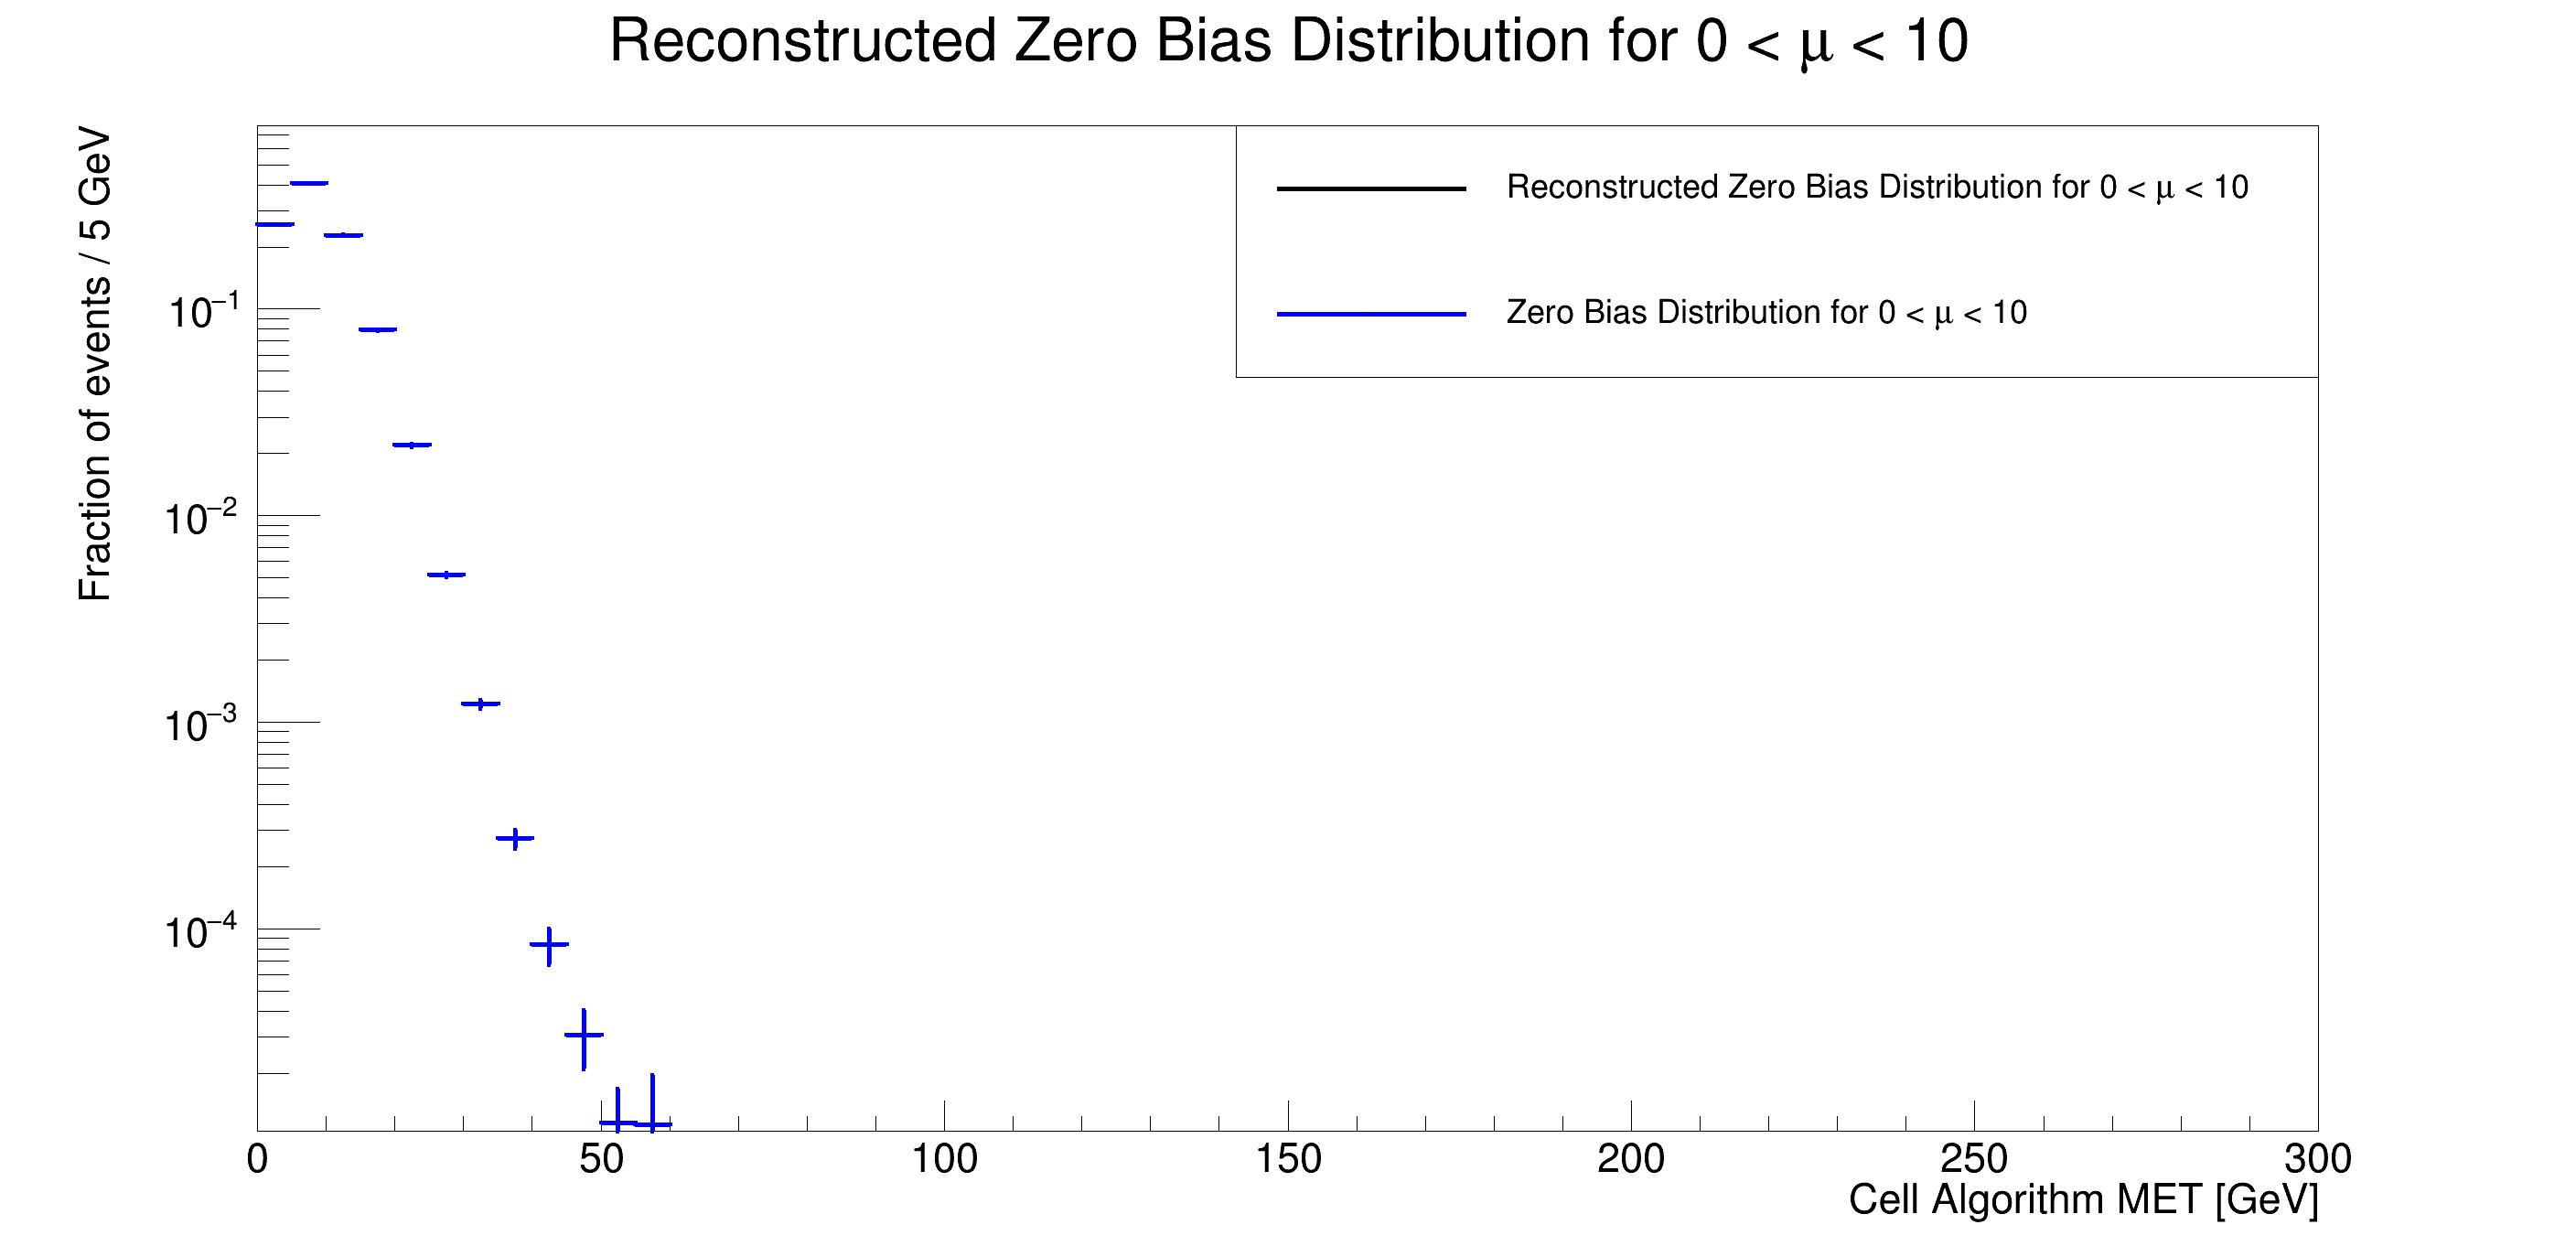
\includegraphics[height=2.65in,width=4.25in]{reconstructed_distributions/reconstructed_distribution_mubin_0}}
\end{frame}
\begin{frame}
		\framebox{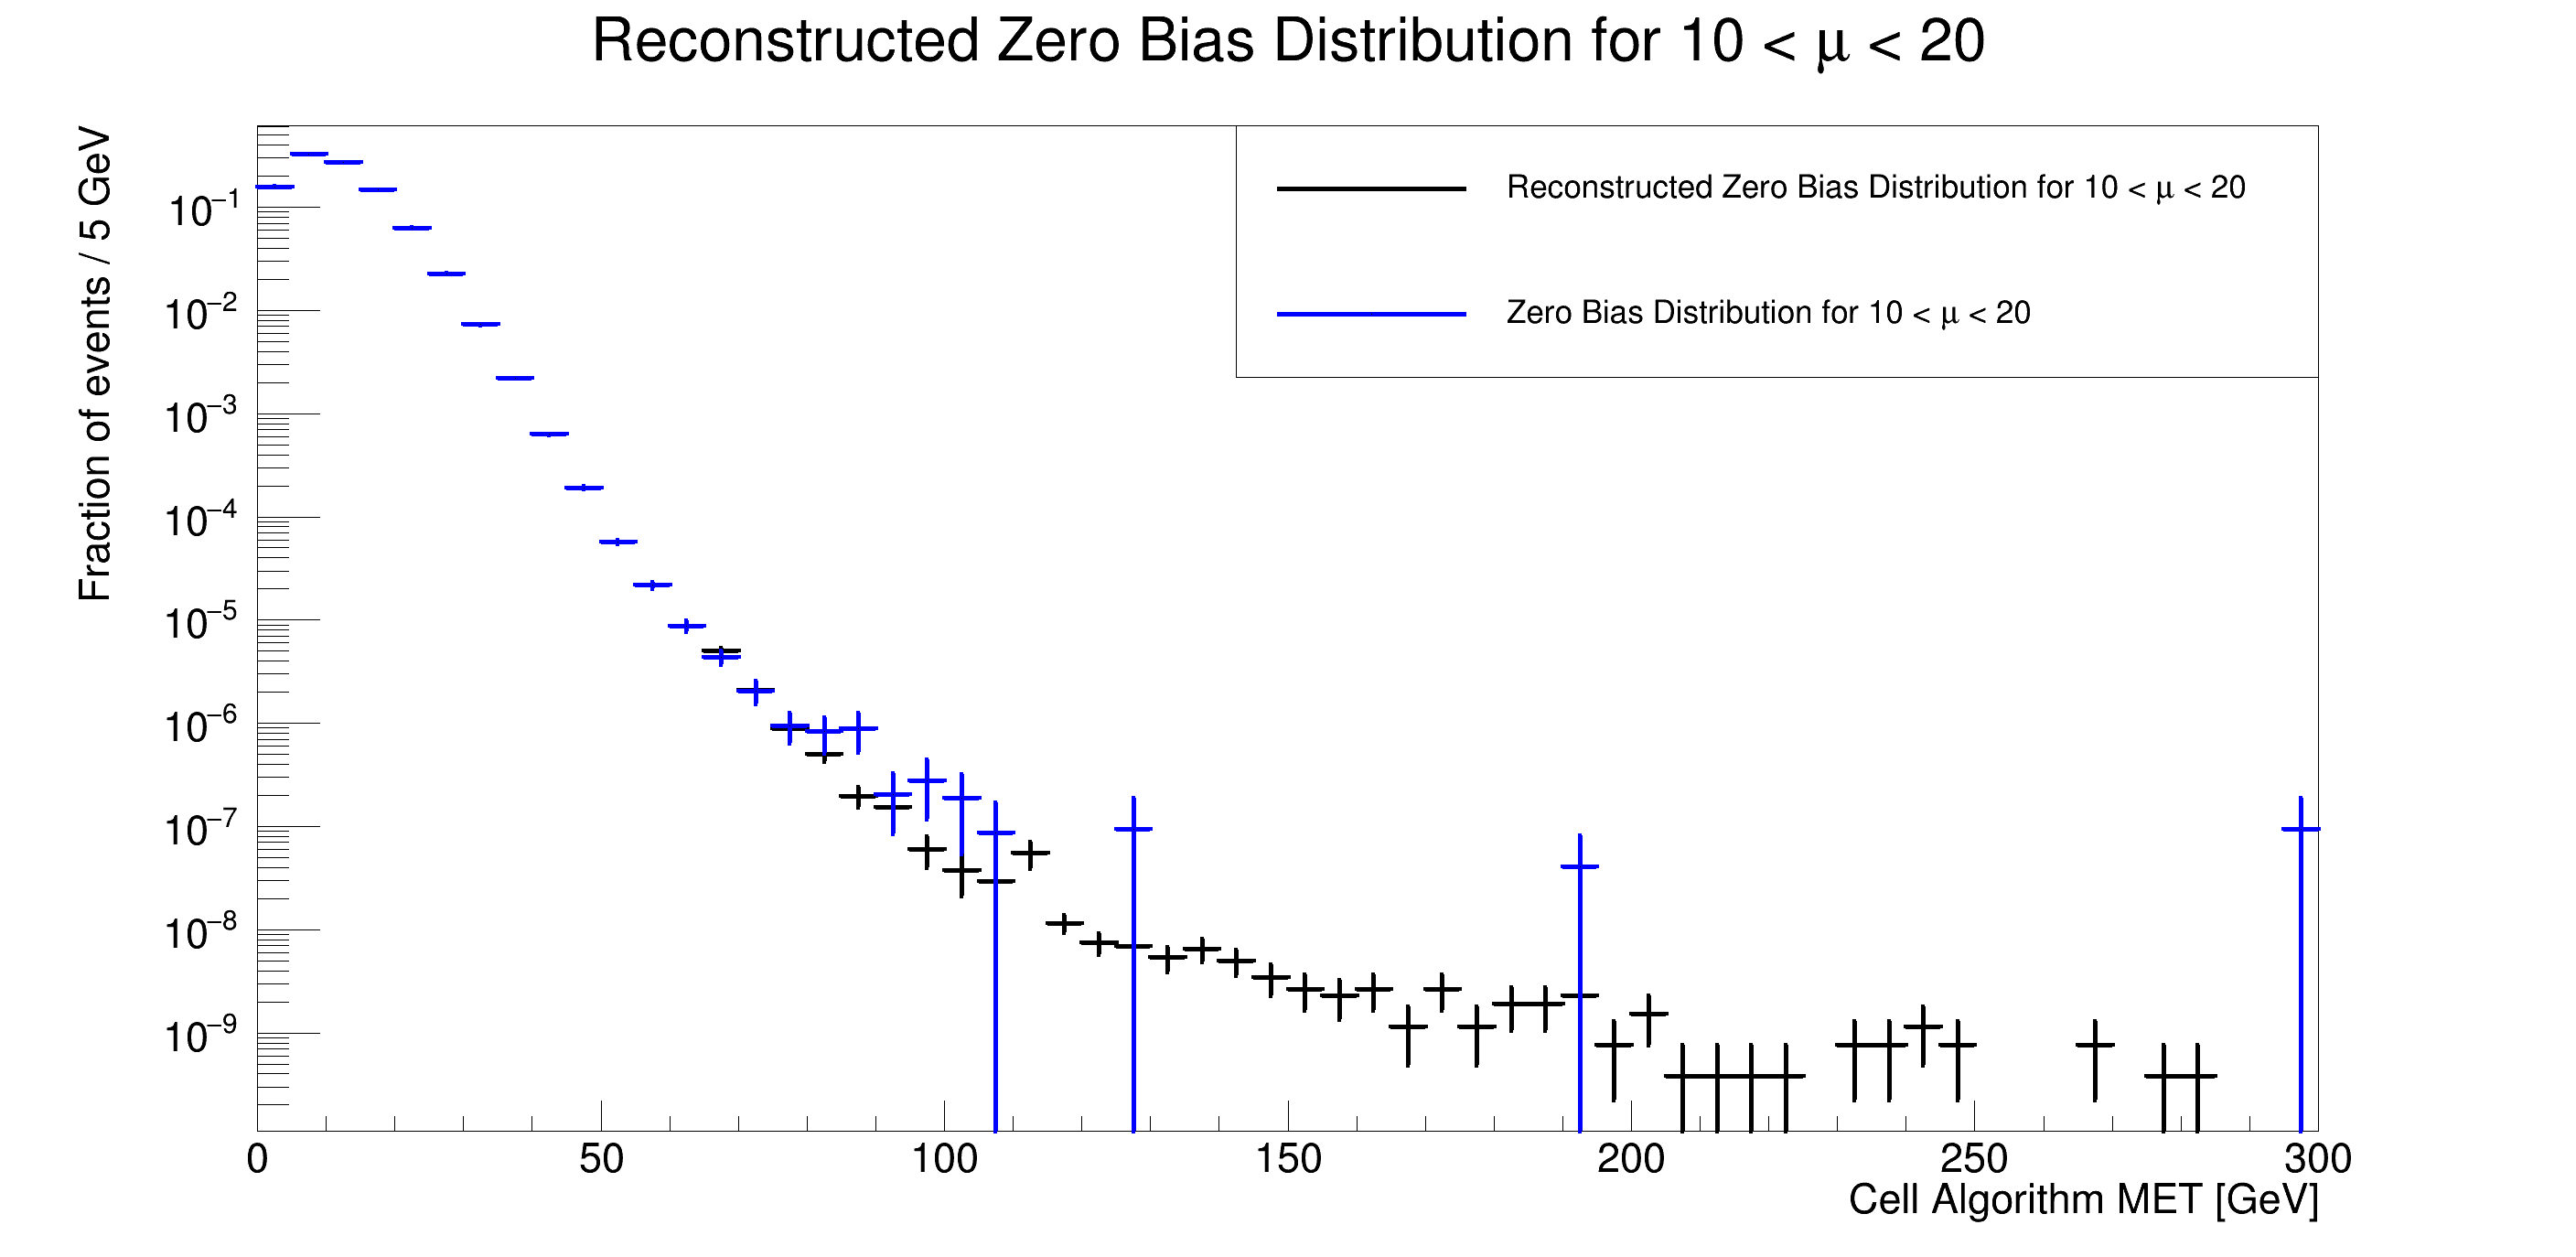
\includegraphics[height=2.65in,width=4.25in]{reconstructed_distributions/reconstructed_distribution_mubin_1}}
\end{frame}
\begin{frame}
		\framebox{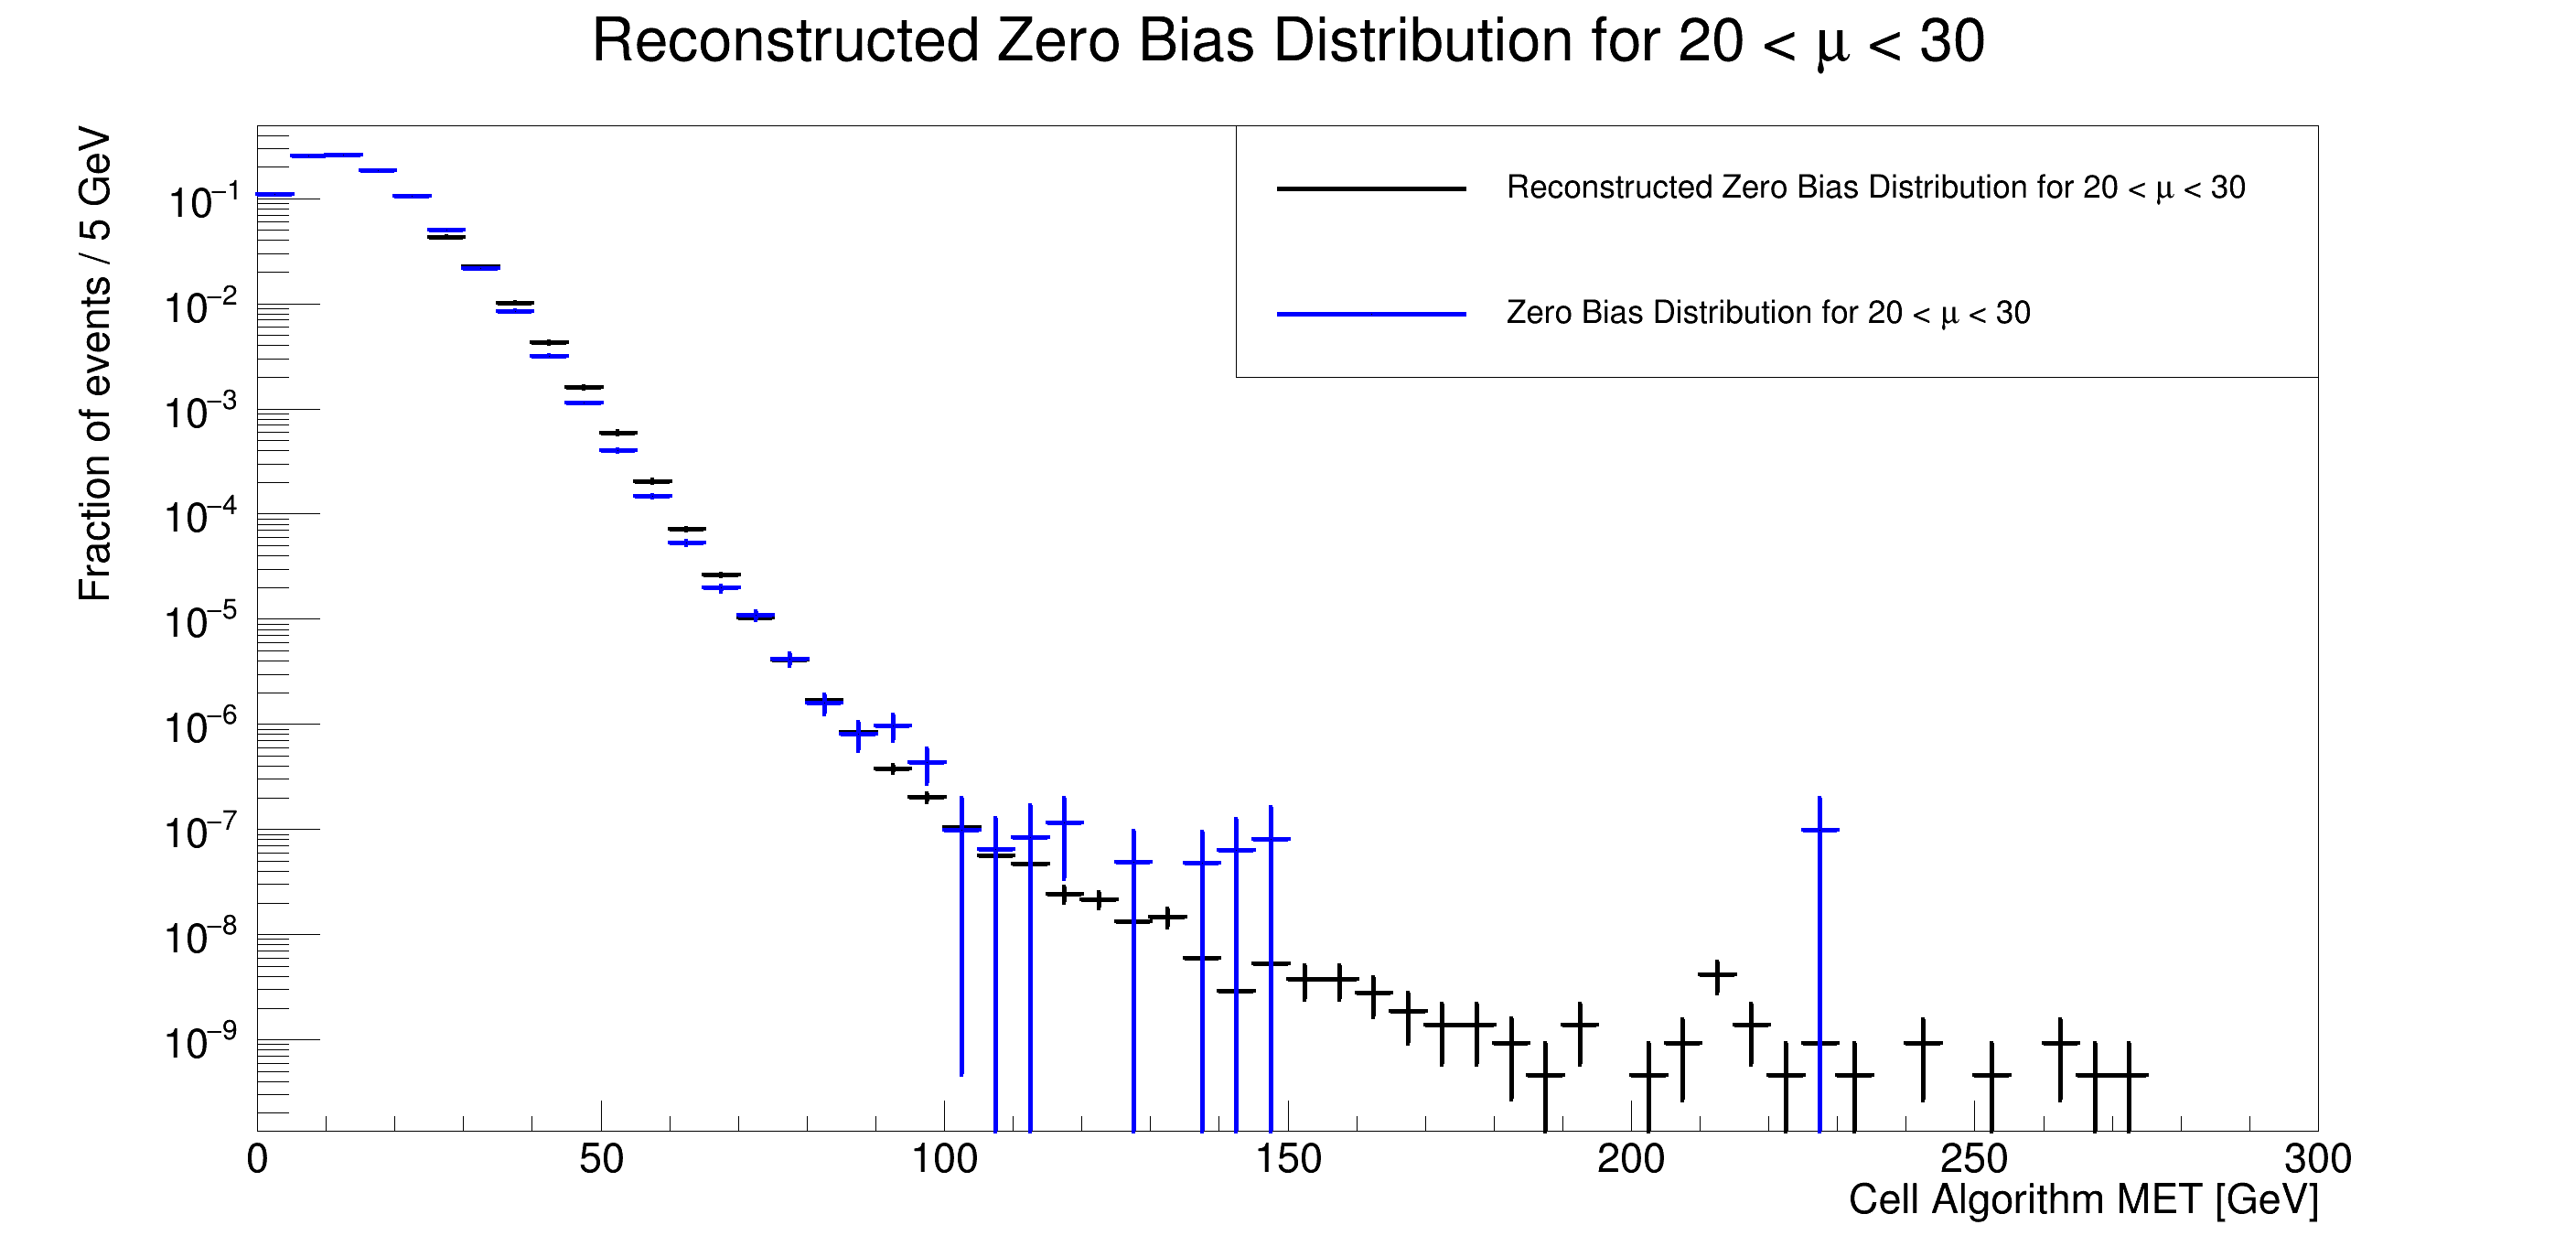
\includegraphics[height=2.65in,width=4.25in]{reconstructed_distributions/reconstructed_distribution_mubin_2}}
\end{frame}
\begin{frame}
		\framebox{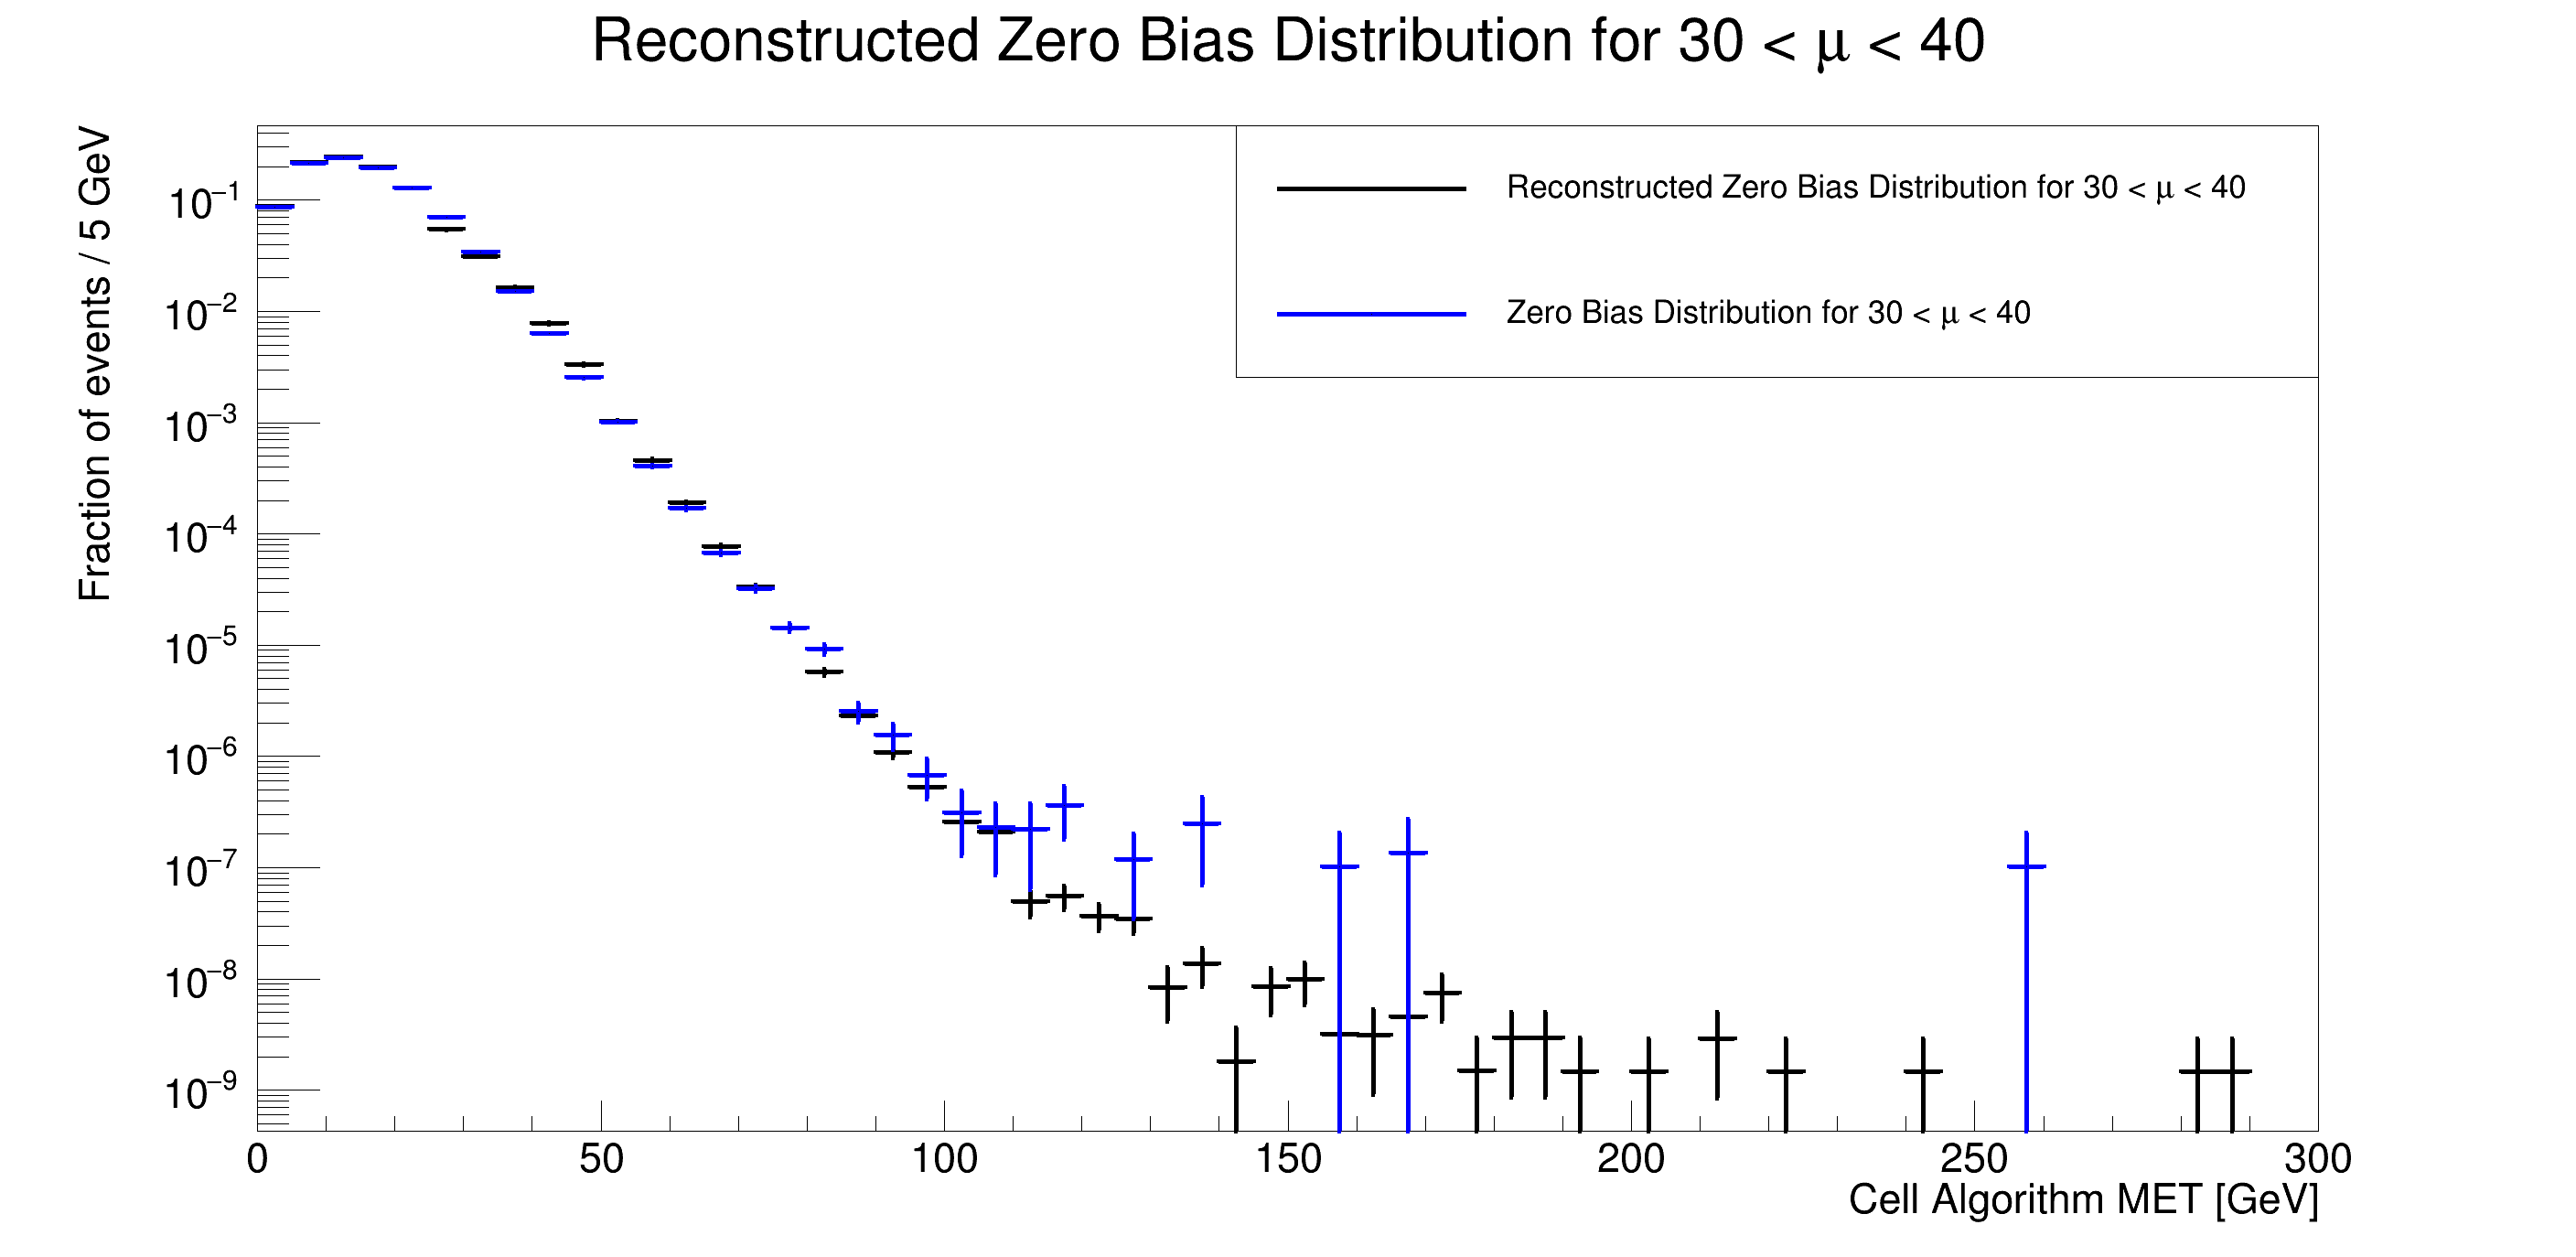
\includegraphics[height=2.65in,width=4.25in]{reconstructed_distributions/reconstructed_distribution_mubin_3}}
\end{frame}
\begin{frame}
		\framebox{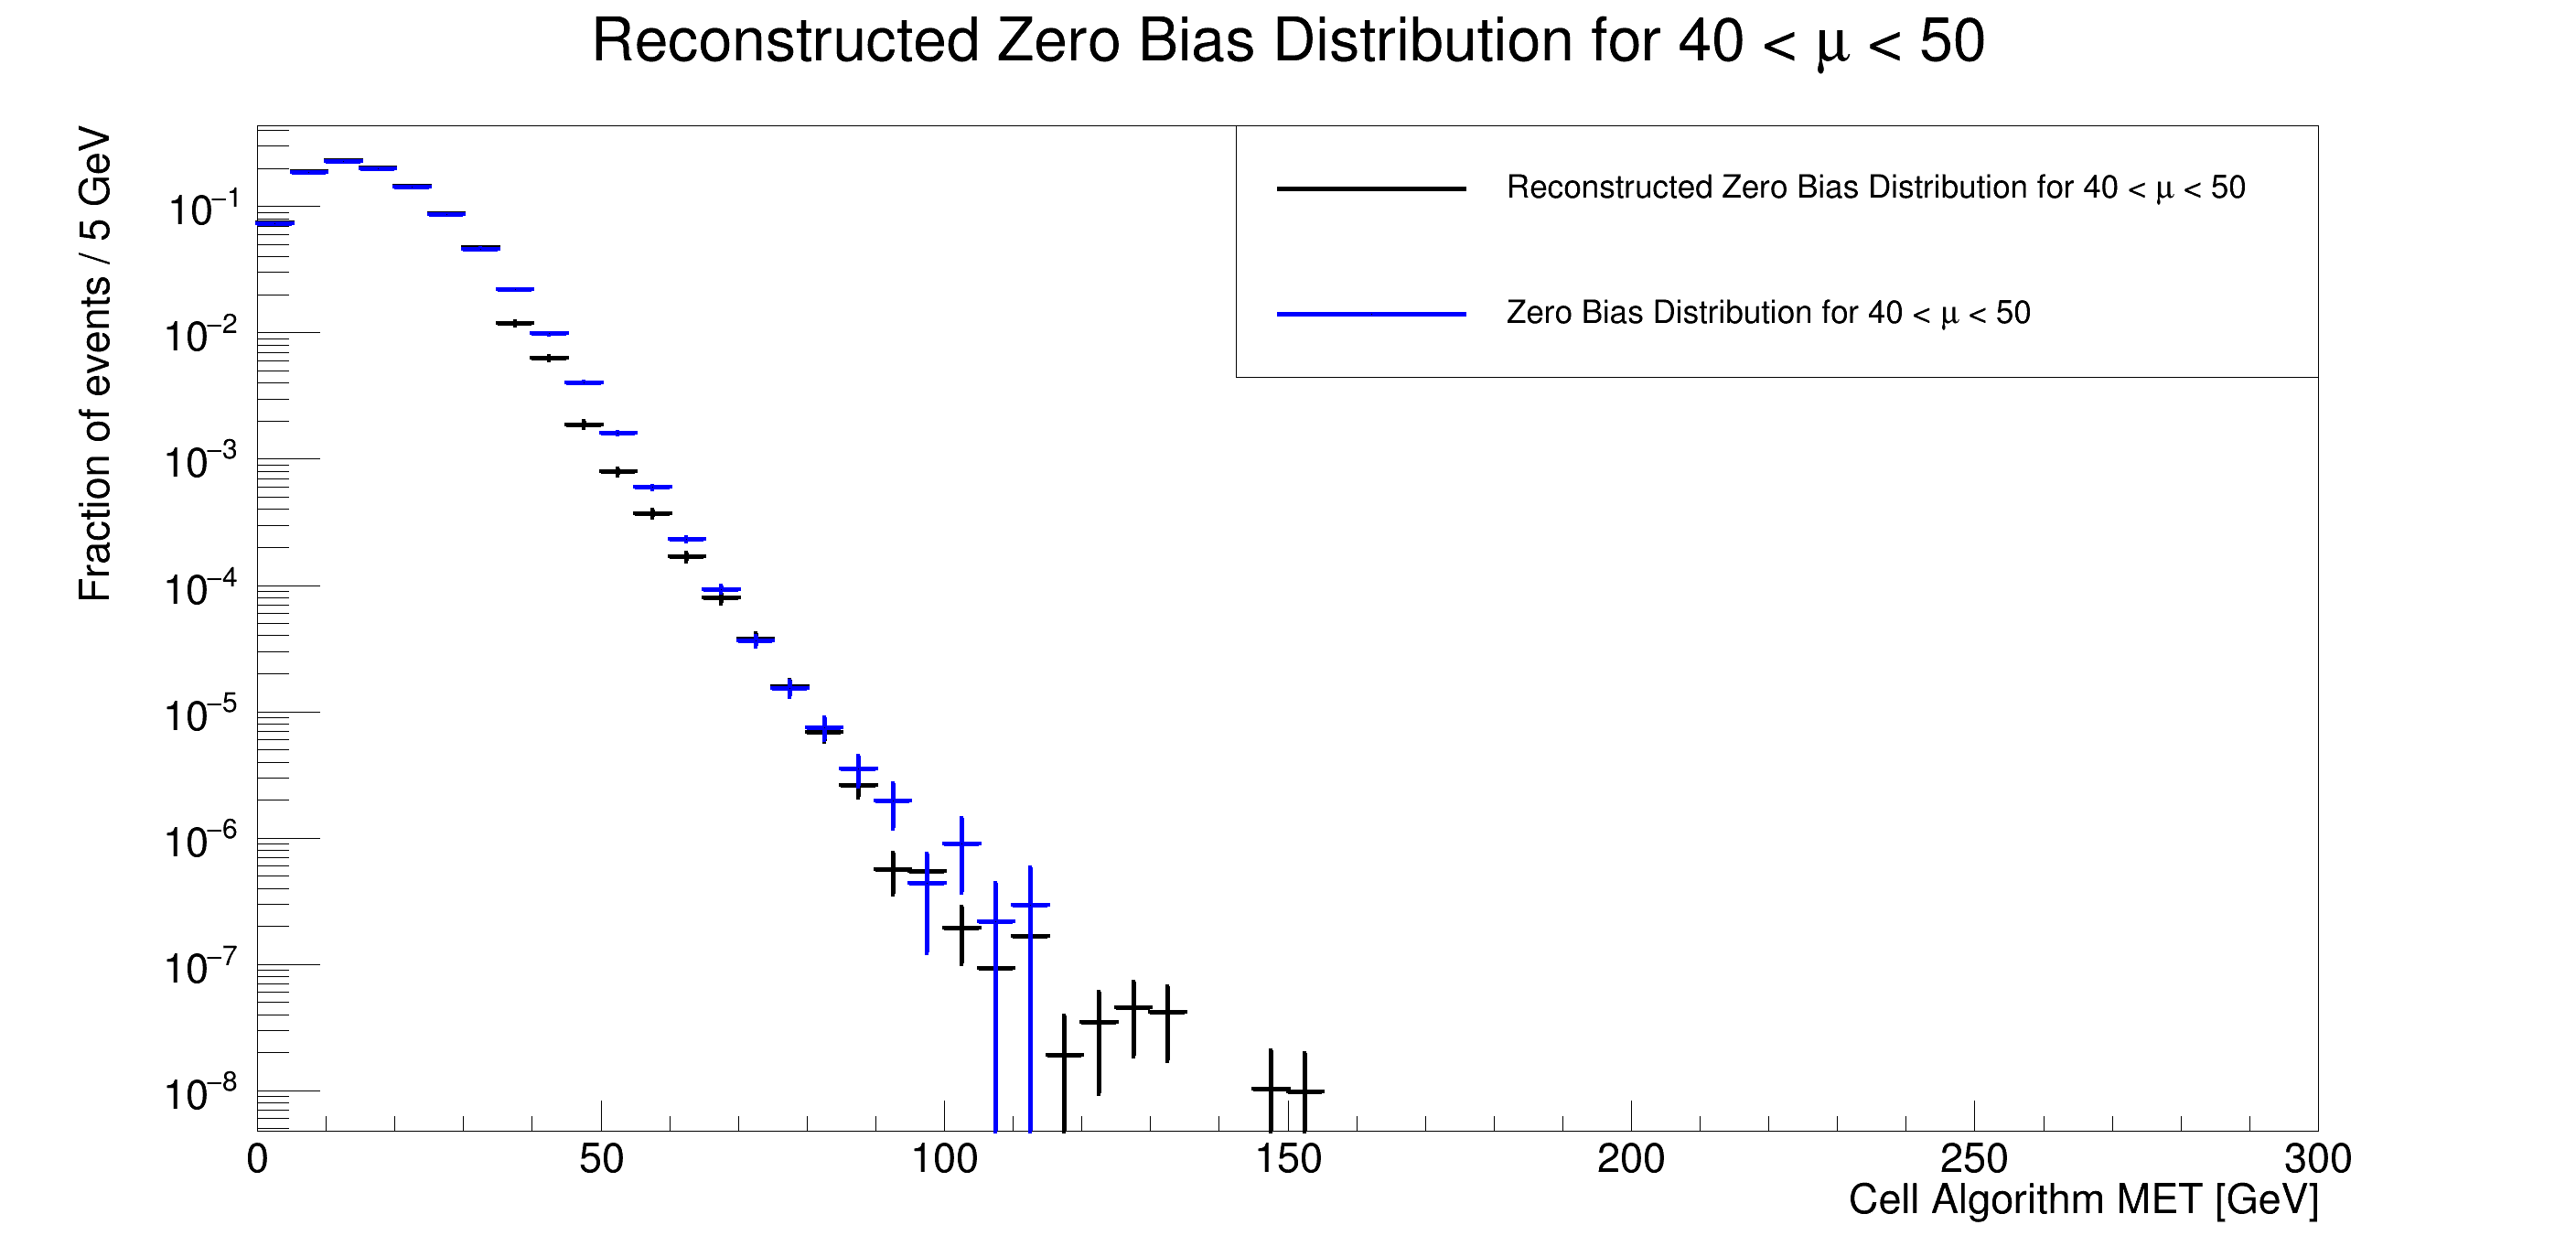
\includegraphics[height=2.65in,width=4.25in]{reconstructed_distributions/reconstructed_distribution_mubin_4}}
\end{frame}
\begin{frame}
		\framebox{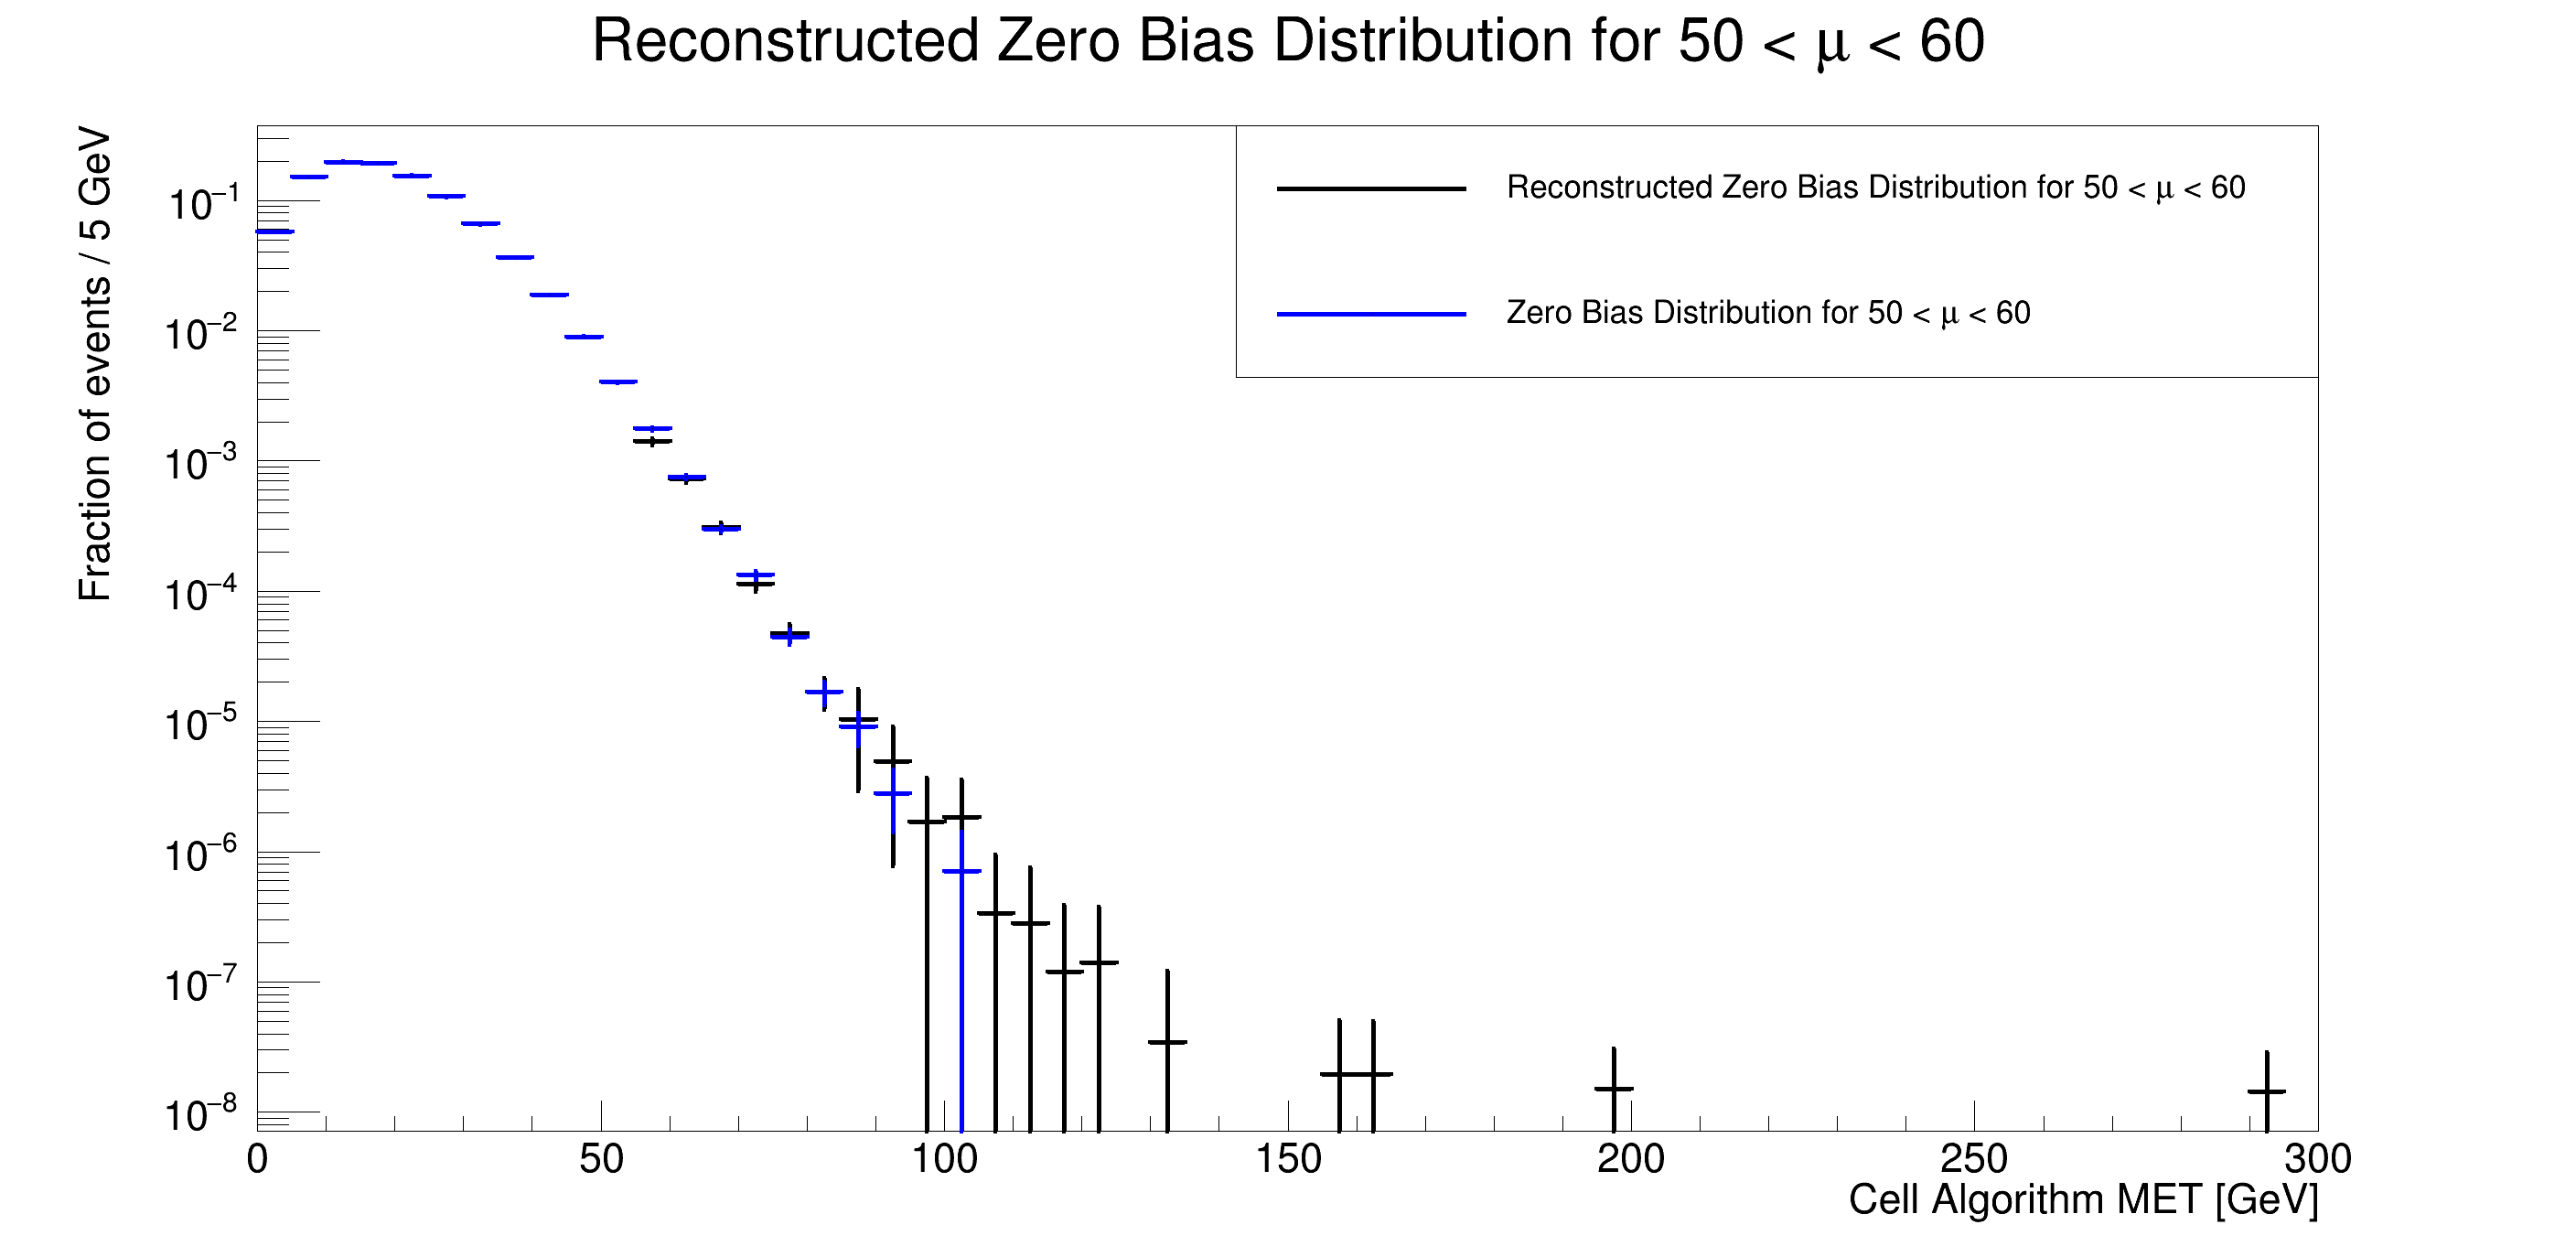
\includegraphics[height=2.65in,width=4.25in]{reconstructed_distributions/reconstructed_distribution_mubin_5}}
\end{frame}
\begin{frame}
		\framebox{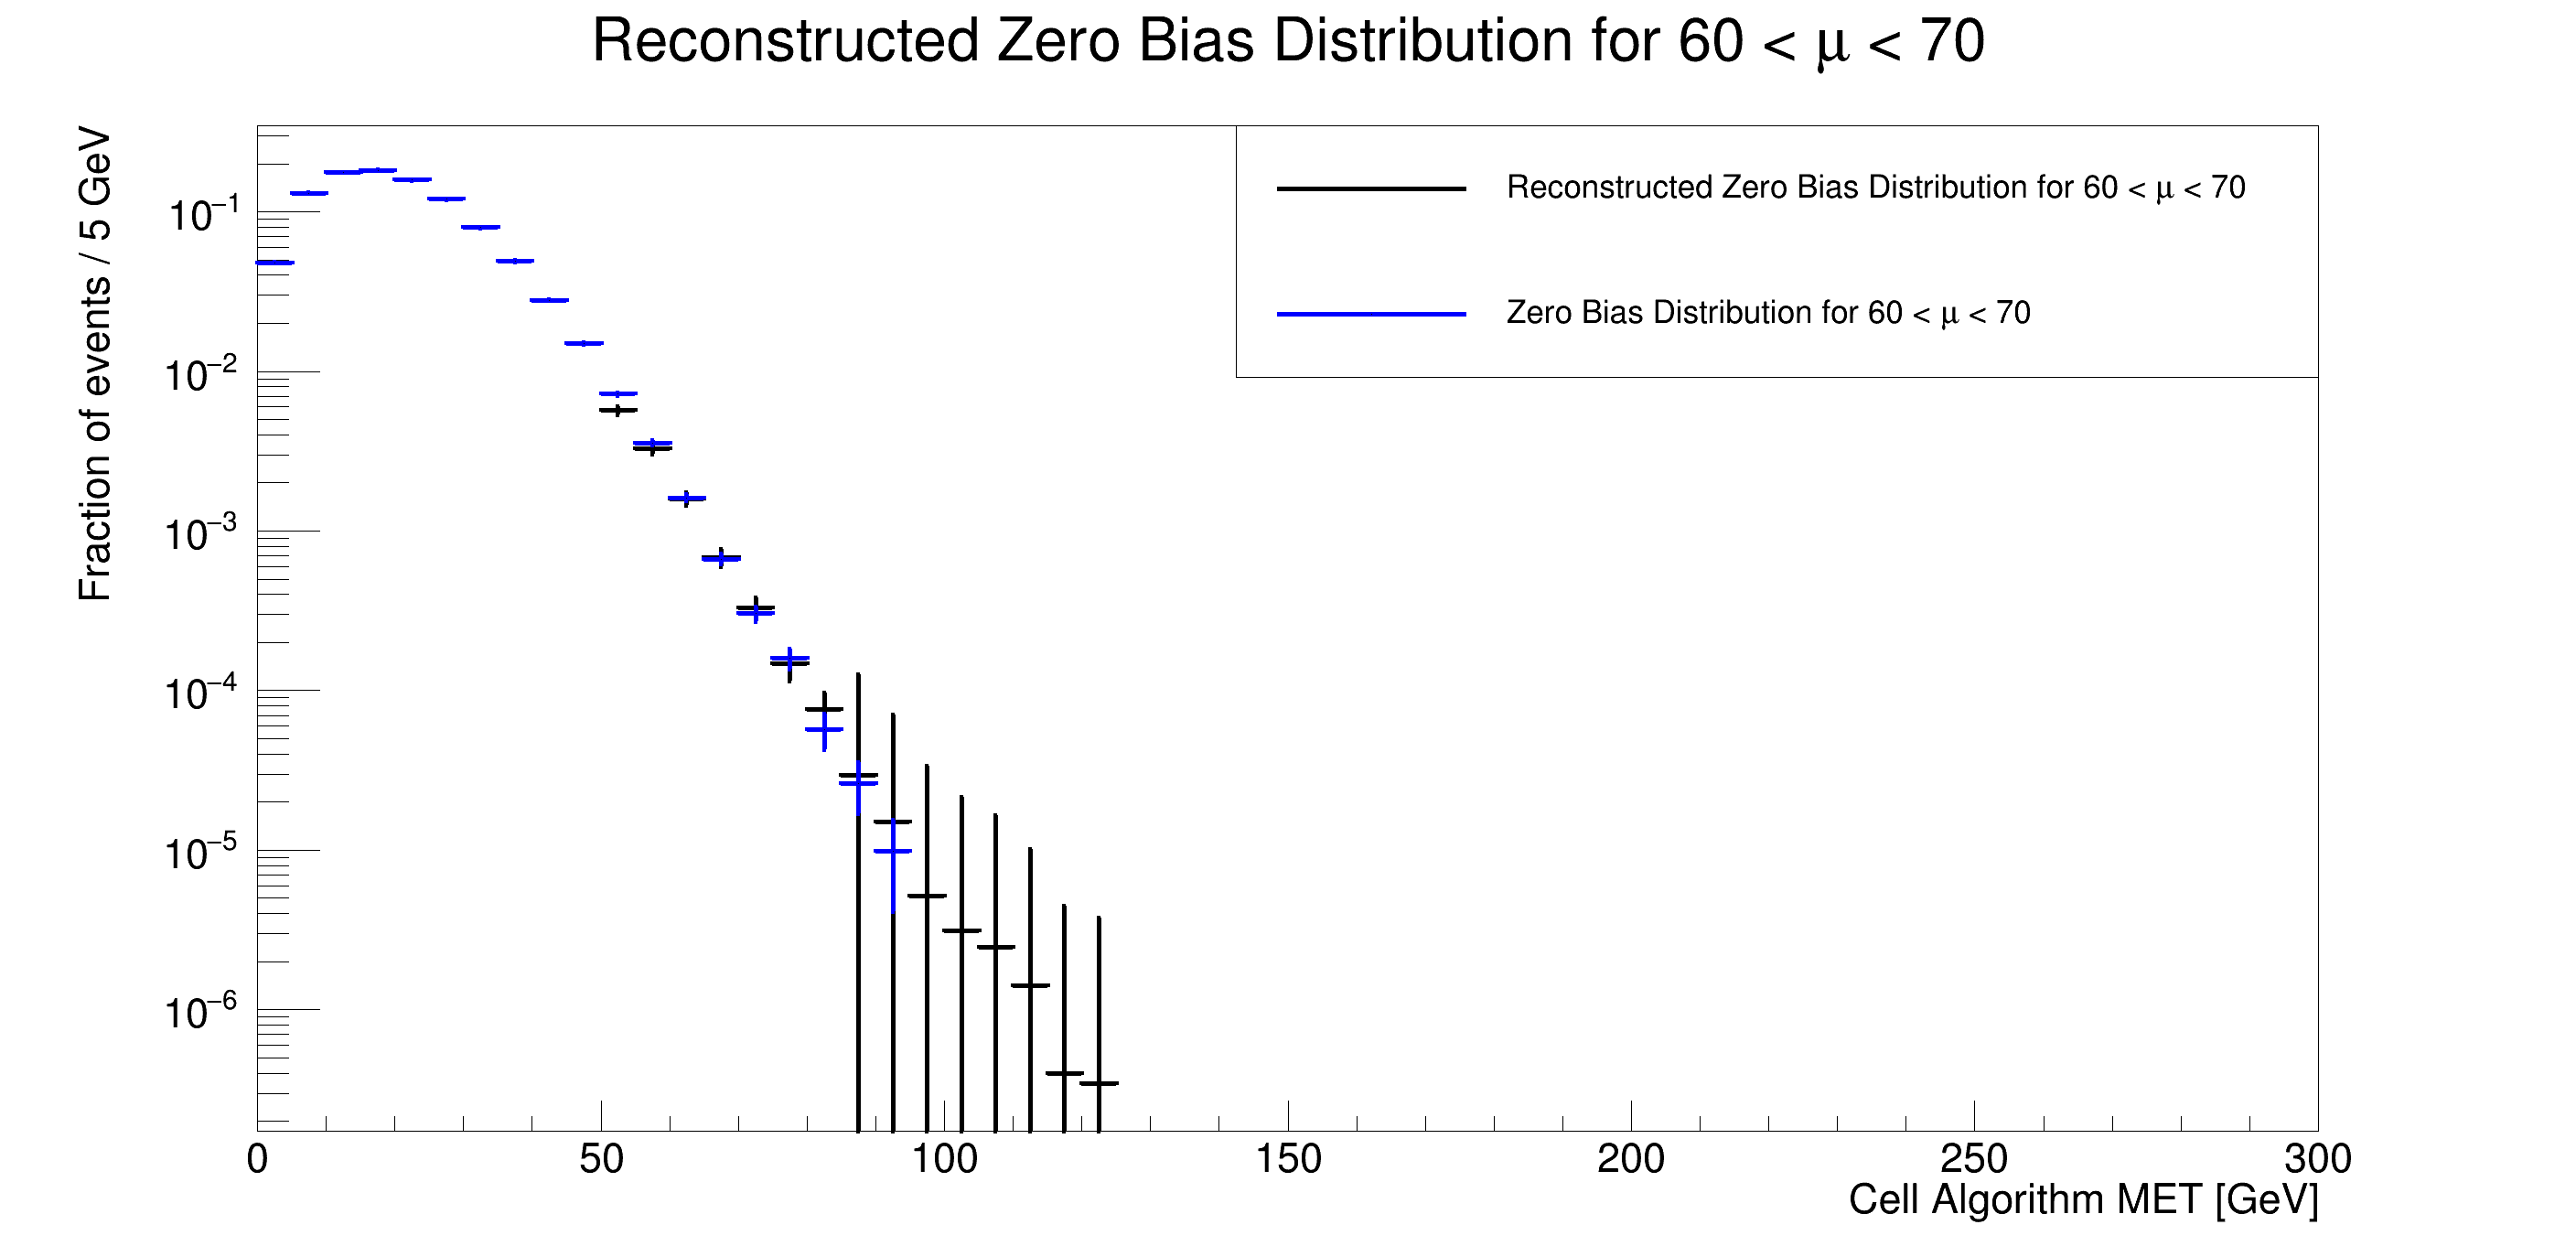
\includegraphics[height=2.65in,width=4.25in]{reconstructed_distributions/reconstructed_distribution_mubin_6}}
\end{frame}
\begin{frame}
\section{Appendix}
\LARGE{Appendix}
\end{frame}

\begin{frame}
        \frametitle{L1XE30 Efficiencies with respect to \texttt{HLTnoalg\_L1ZB} Data}
		\framebox{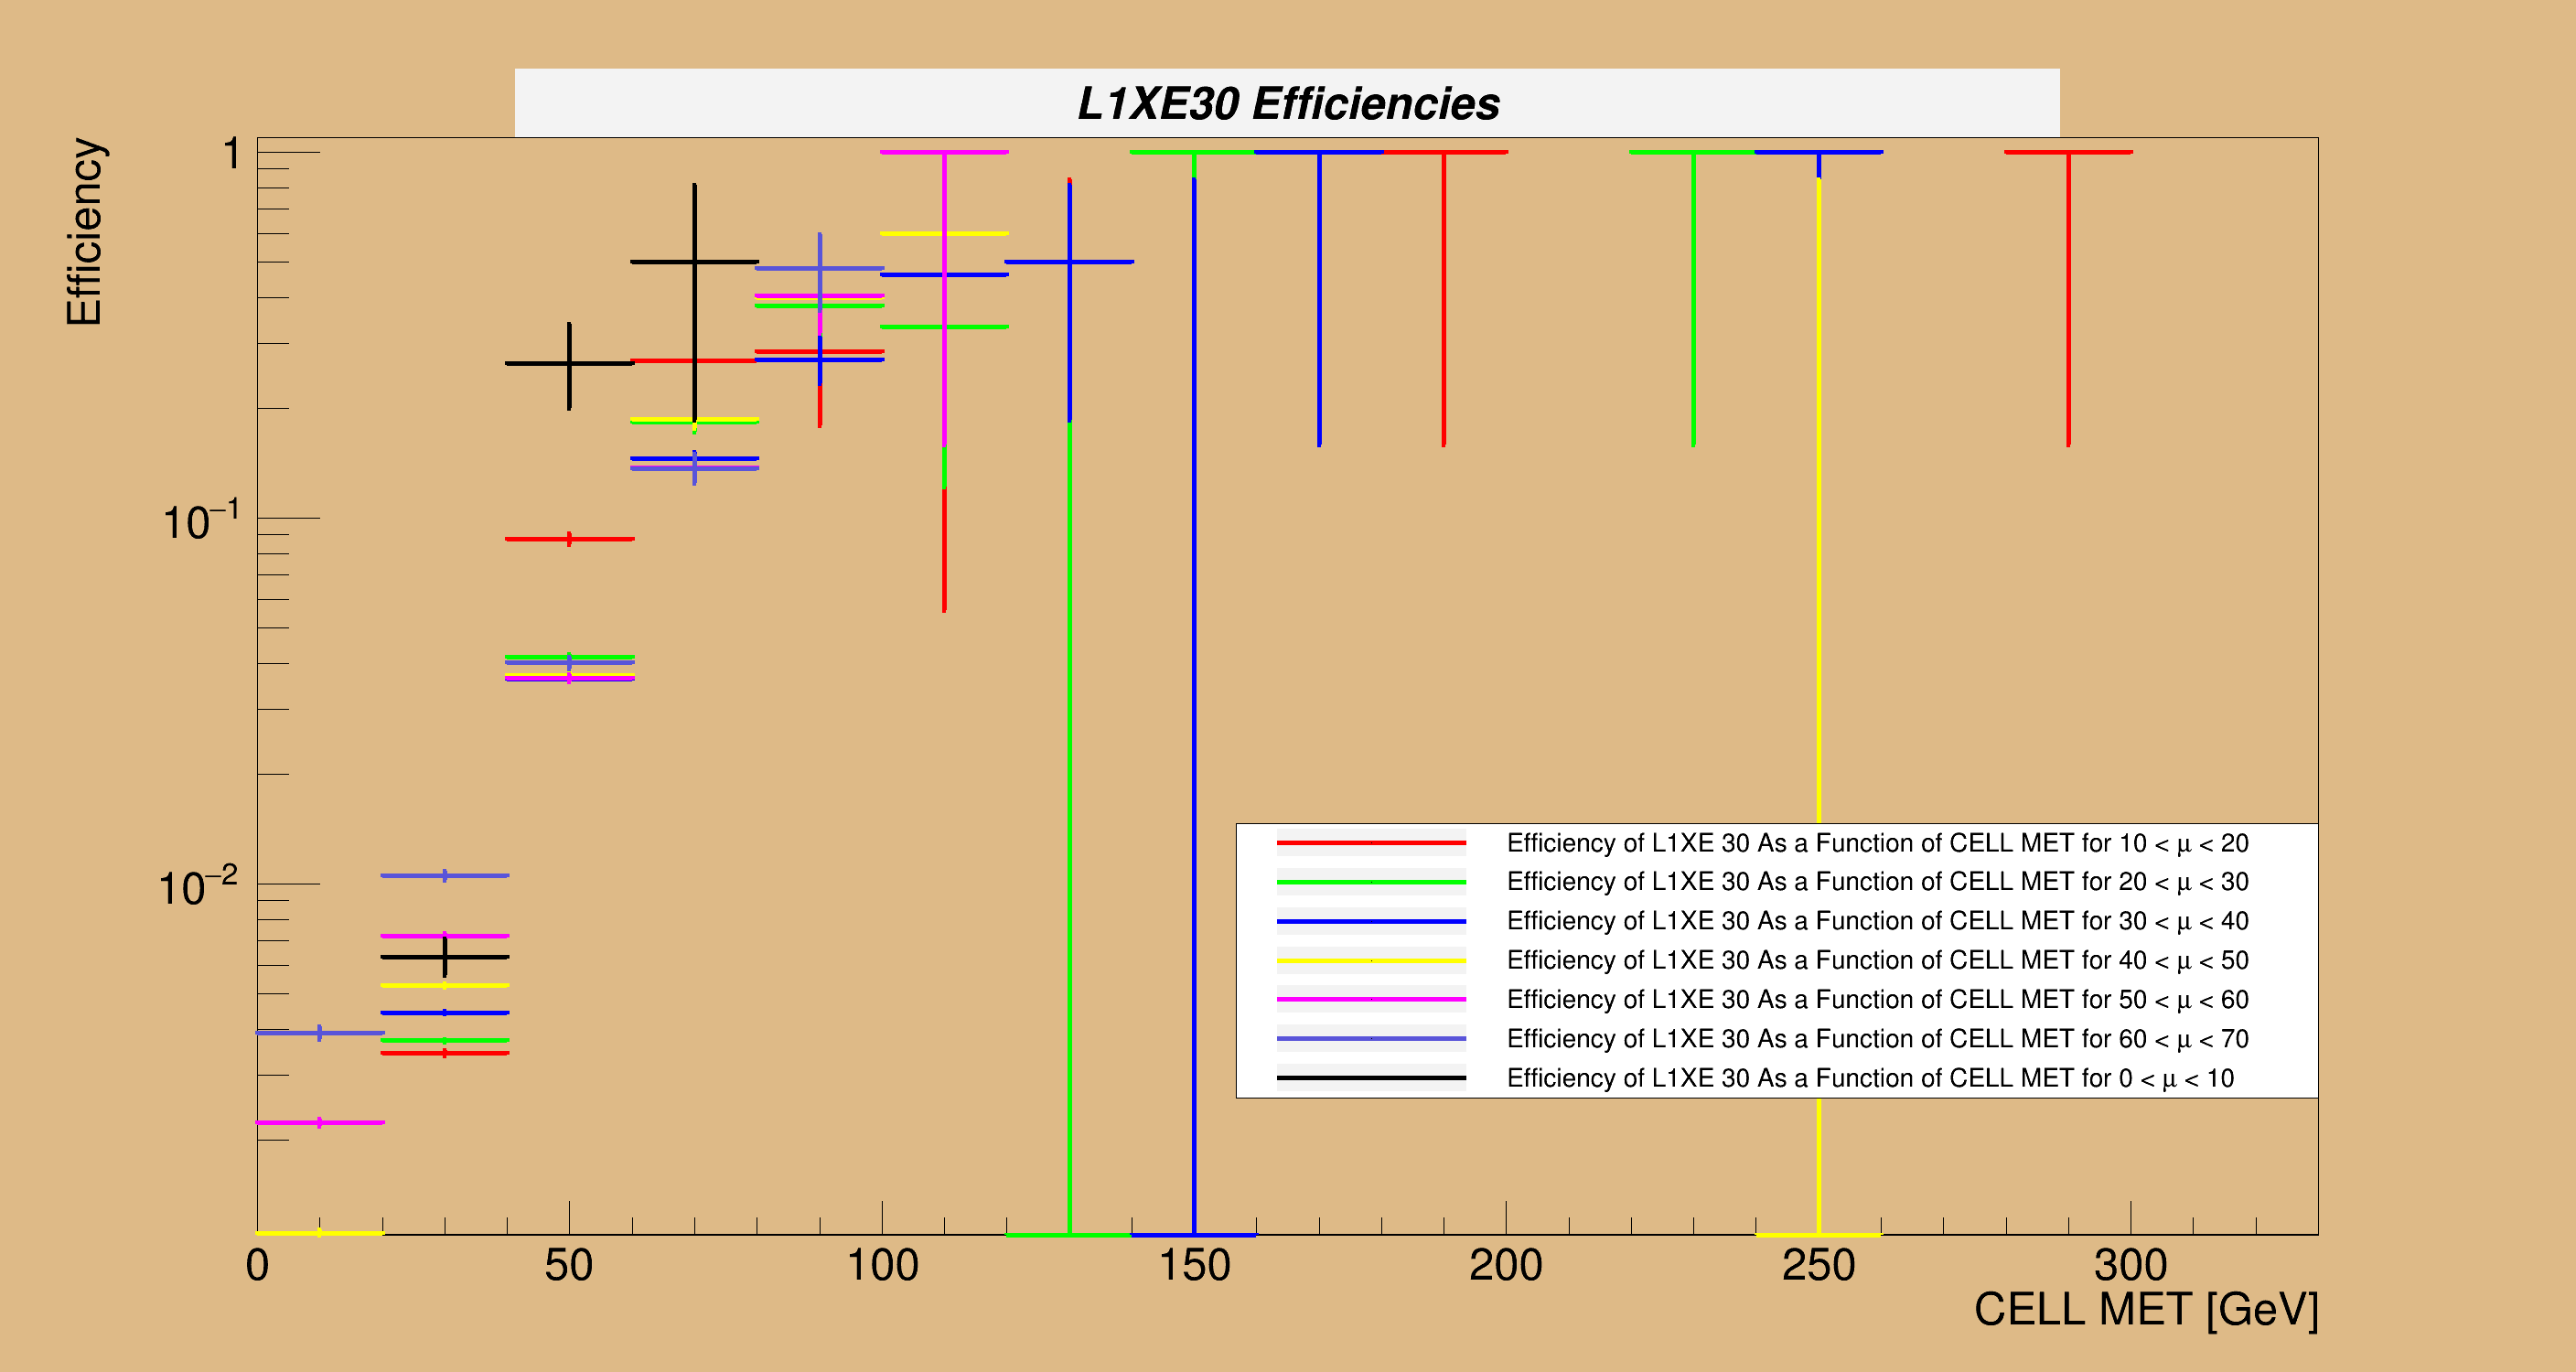
\includegraphics[height=2.65in,width=4.25in]{L1XE30Efficiency_Curves}}
\end{frame}
\begin{frame}
        \frametitle{L1XE50 Efficiencies with respect to \texttt{HLTnoalg\_L1XE30} Data}
		\framebox{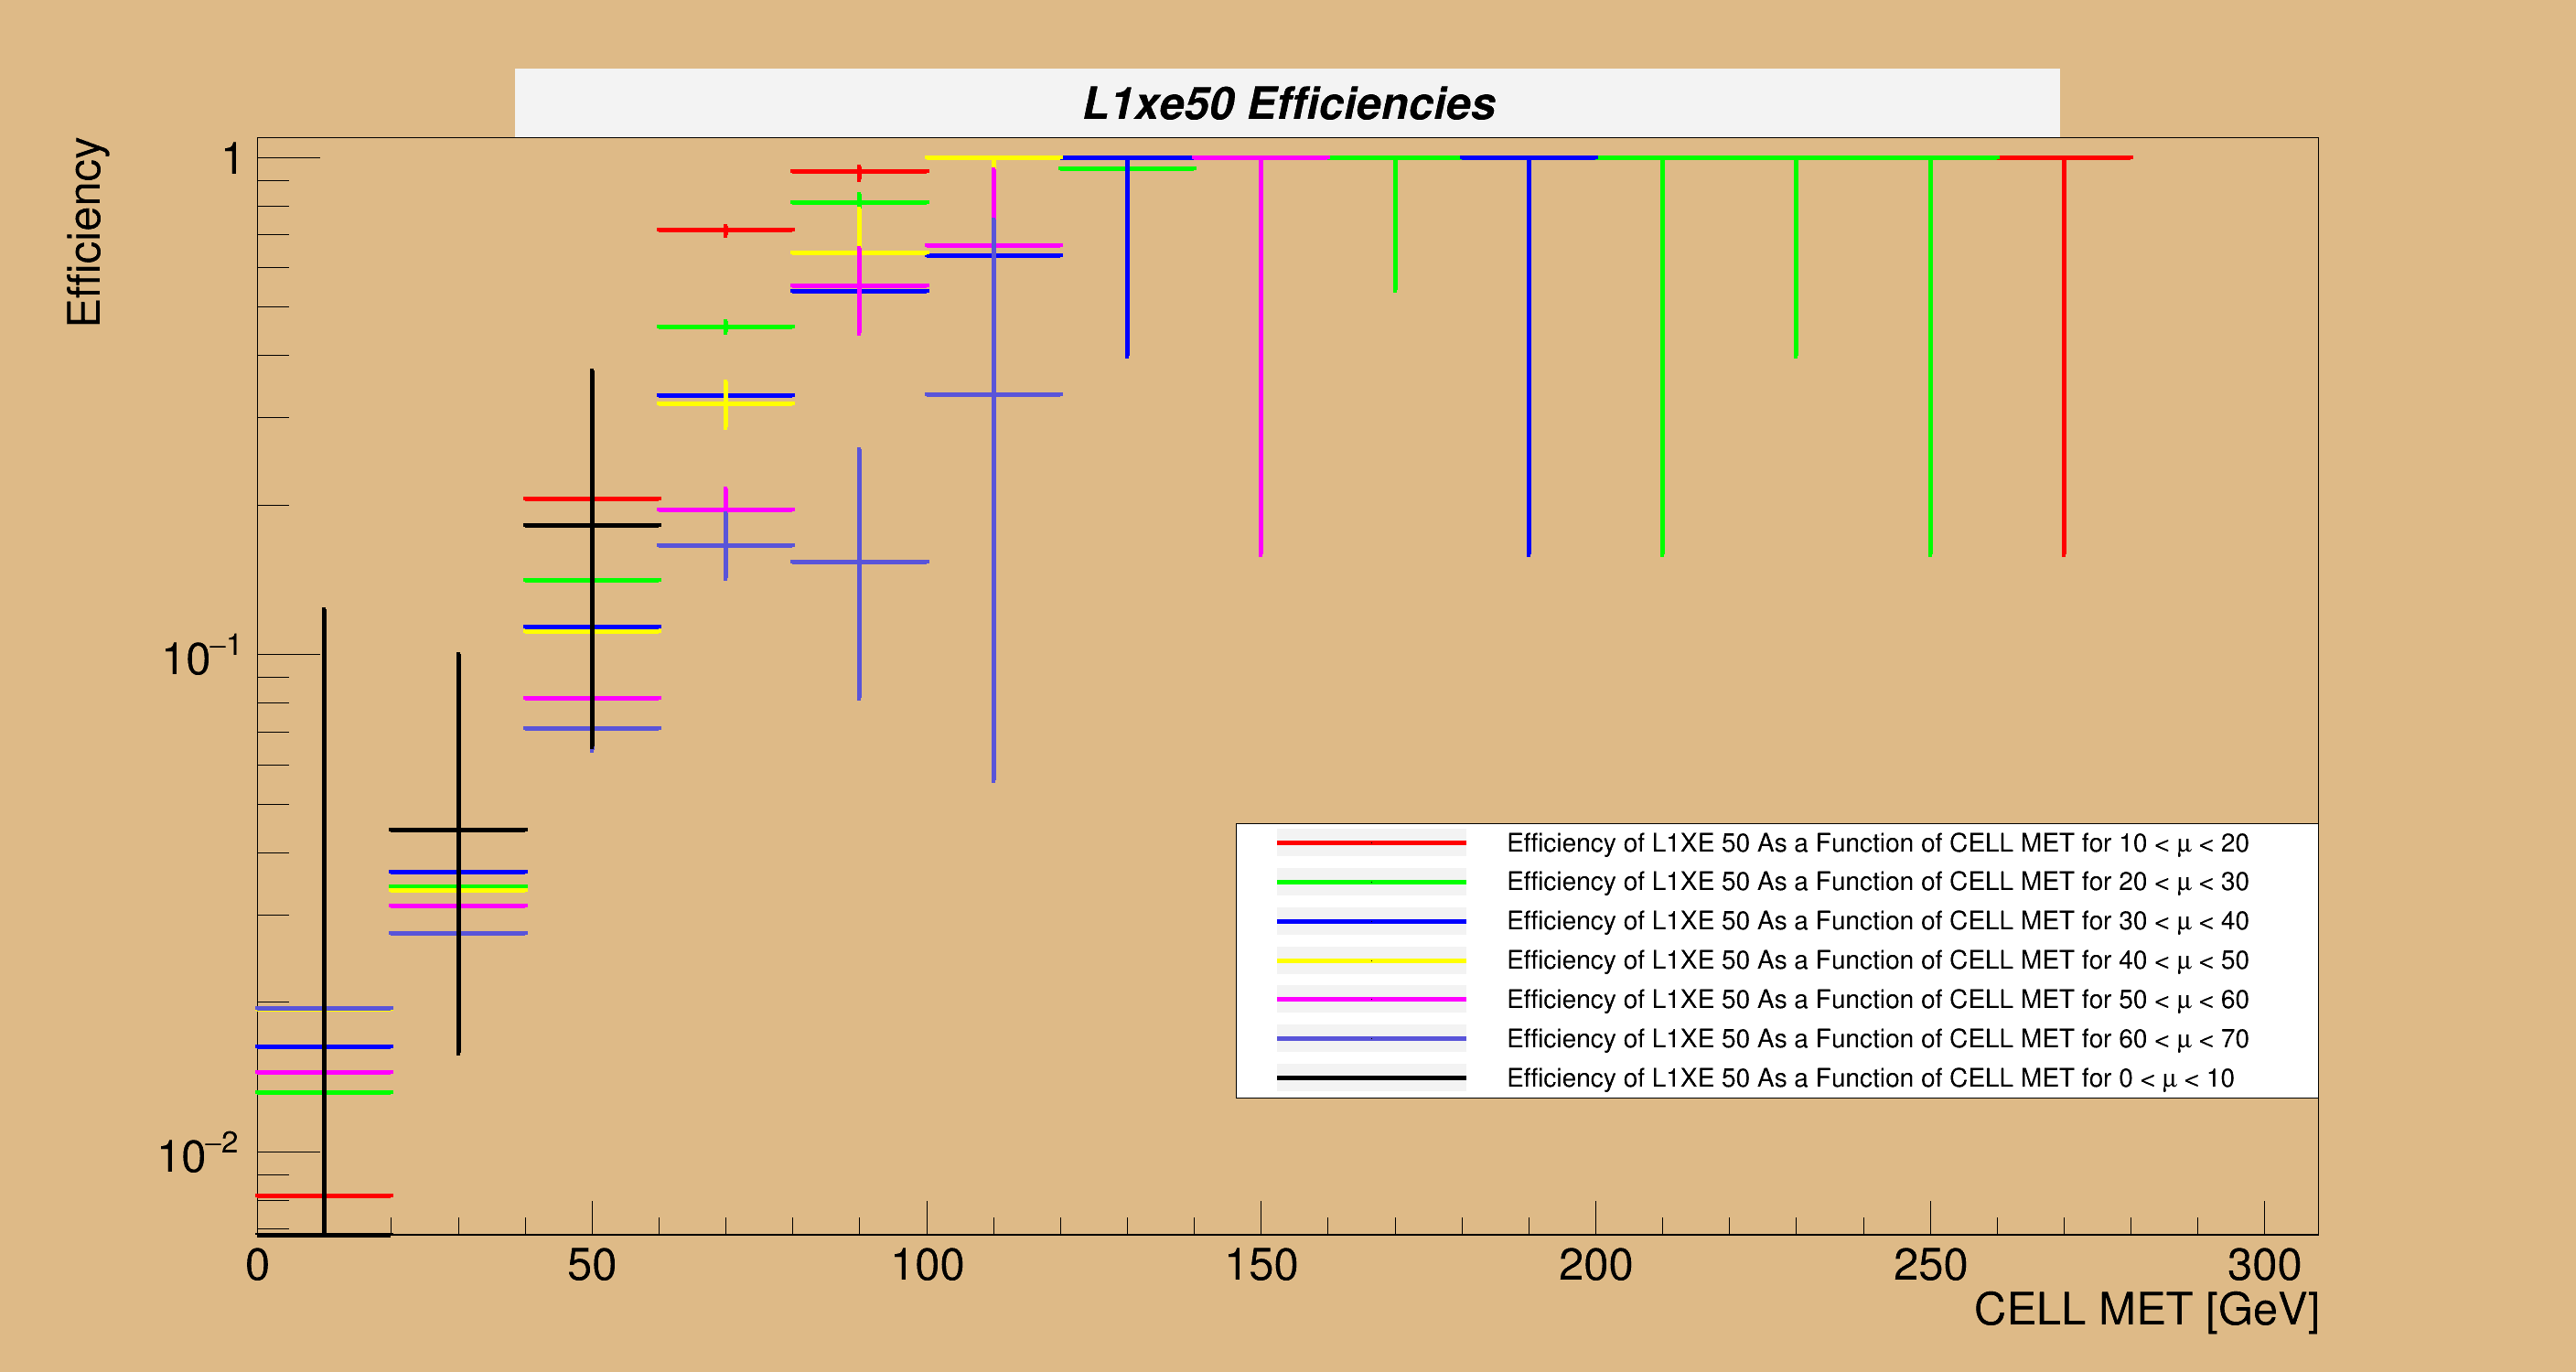
\includegraphics[height=2.65in,width=4.25in]{L1XE50Efficiency_Curves}}
\end{frame}
% HLTNOALG L1XE30 Plots
\begin{frame}
        \frametitle{\texttt{HLTnoalg\_L1XE30} Plot for $0<\mu<10$}
        \framebox{\includegraphics[height=2.65in,width=4.25in]{hlt_noalg_l1xe30_plots/hlt_noalg_L1XE30_dist_mubin_0}}
\end{frame}
\begin{frame}
        \frametitle{\texttt{HLTnoalg\_L1XE30} Plot for $10<\mu<20$}
        \framebox{\includegraphics[height=2.65in,width=4.25in]{hlt_noalg_l1xe30_plots/hlt_noalg_L1XE30_dist_mubin_1}}
\end{frame}
\begin{frame}
        \frametitle{\texttt{HLTnoalg\_L1XE30} Plot for $20<\mu<30$}
        \framebox{\includegraphics[height=2.65in,width=4.25in]{hlt_noalg_l1xe30_plots/hlt_noalg_L1XE30_dist_mubin_2}}
\end{frame}
\begin{frame}
        \frametitle{\texttt{HLTnoalg\_L1XE30} Plot for $30<\mu<40$}
        \framebox{\includegraphics[height=2.65in,width=4.25in]{hlt_noalg_l1xe30_plots/hlt_noalg_L1XE30_dist_mubin_3}}
\end{frame}
\begin{frame}
        \frametitle{\texttt{HLTnoalg\_L1XE30} Plot for $40<\mu<50$}
        \framebox{\includegraphics[height=2.65in,width=4.25in]{hlt_noalg_l1xe30_plots/hlt_noalg_L1XE30_dist_mubin_4}}
\end{frame}
\begin{frame}
        \frametitle{\texttt{HLTnoalg\_L1XE30} Plot for $50<\mu<60$}
        \framebox{\includegraphics[height=2.65in,width=4.25in]{hlt_noalg_l1xe30_plots/hlt_noalg_L1XE30_dist_mubin_5}}
\end{frame}
\begin{frame}
        \frametitle{\texttt{HLTnoalg\_L1XE30} Plot for $60<\mu<70$}
        \framebox{\includegraphics[height=2.65in,width=4.25in]{hlt_noalg_l1xe30_plots/hlt_noalg_L1XE30_dist_mubin_6}}
\end{frame}
% HLTNOALG L1XE50 Plots
\begin{frame}
        \frametitle{\texttt{HLTnoalg\_L1XE50} Plot for $0<\mu<10$}
        \framebox{\includegraphics[height=2.65in,width=4.25in]{hlt_noalg_l1xe50_plots/hlt_noalg_L1XE50_dist_mubin_0}}
\end{frame}
\begin{frame}
        \frametitle{\texttt{HLTnoalg\_L1XE50} Plot for $10<\mu<20$}
        \framebox{\includegraphics[height=2.65in,width=4.25in]{hlt_noalg_l1xe50_plots/hlt_noalg_L1XE50_dist_mubin_1}}
\end{frame}
\begin{frame}
        \frametitle{\texttt{HLTnoalg\_L1XE50} Plot for $20<\mu<30$}
        \framebox{\includegraphics[height=2.65in,width=4.25in]{hlt_noalg_l1xe50_plots/hlt_noalg_L1XE50_dist_mubin_2}}
\end{frame}
\begin{frame}
        \frametitle{\texttt{HLTnoalg\_L1XE50} Plot for $30<\mu<40$}
        \framebox{\includegraphics[height=2.65in,width=4.25in]{hlt_noalg_l1xe50_plots/hlt_noalg_L1XE50_dist_mubin_3}}
\end{frame}
\begin{frame}
        \frametitle{\texttt{HLTnoalg\_L1XE50} Plot for $40<\mu<50$}
        \framebox{\includegraphics[height=2.65in,width=4.25in]{hlt_noalg_l1xe50_plots/hlt_noalg_L1XE50_dist_mubin_4}}
\end{frame}
\begin{frame}
        \frametitle{\texttt{HLTnoalg\_L1XE50} Plot for $50<\mu<60$}
        \framebox{\includegraphics[height=2.65in,width=4.25in]{hlt_noalg_l1xe50_plots/hlt_noalg_L1XE50_dist_mubin_5}}
\end{frame}
\begin{frame}
        \frametitle{\texttt{HLTnoalg\_L1XE50} Plot for $60<\mu<70$}
        \framebox{\includegraphics[height=2.65in,width=4.25in]{hlt_noalg_l1xe50_plots/hlt_noalg_L1XE50_dist_mubin_6}}
\end{frame}
% L1XE30 Efficiency Curves
\begin{frame}
        \frametitle{L1XE30 Efficiency Curve Plot for $0<\mu<10$}
        \framebox{\includegraphics[height=2.65in,width=4.25in]{l1xe30_efficiencies/L1XE30Efficiency_mu_between_0_10}}
\end{frame}
\begin{frame}
        \frametitle{L1XE30 Efficiency Curve Plot for $10<\mu<20$}
        \framebox{\includegraphics[height=2.65in,width=4.25in]{l1xe30_efficiencies/L1XE30Efficiency_mu_between_10_20}}
\end{frame}
\begin{frame}
        \frametitle{L1XE30 Efficiency Curve Plot for $20<\mu<30$}
        \framebox{\includegraphics[height=2.65in,width=4.25in]{l1xe30_efficiencies/L1XE30Efficiency_mu_between_20_30}}
\end{frame}
\begin{frame}
        \frametitle{L1XE30 Efficiency Curve Plot for $30<\mu<40$}
        \framebox{\includegraphics[height=2.65in,width=4.25in]{l1xe30_efficiencies/L1XE30Efficiency_mu_between_30_40}}
\end{frame}
\begin{frame}
        \frametitle{L1XE30 Efficiency Curve Plot for $40<\mu<50$}
        \framebox{\includegraphics[height=2.65in,width=4.25in]{l1xe30_efficiencies/L1XE30Efficiency_mu_between_40_50}}
\end{frame}
\begin{frame}
        \frametitle{L1XE30 Efficiency Curve Plot for $50<\mu<60$}
        \framebox{\includegraphics[height=2.65in,width=4.25in]{l1xe30_efficiencies/L1XE30Efficiency_mu_between_50_60}}
\end{frame}
\begin{frame}
        \frametitle{L1XE30 Efficiency Curve Plot for $60<\mu<70$}
        \framebox{\includegraphics[height=2.65in,width=4.25in]{l1xe30_efficiencies/L1XE30Efficiency_mu_between_60_70}}
\end{frame}
% L1XE50 Efficiency Curves
\begin{frame}
        \frametitle{L1XE50 Efficiency Curve Plot for $0<\mu<10$}
        \framebox{\includegraphics[height=2.65in,width=4.25in]{l1xe50_efficiencies/L1XE50Efficiency_mu_between_0_10}}
\end{frame}
\begin{frame}
        \frametitle{L1XE50 Efficiency Curve Plot for $10<\mu<20$}
        \framebox{\includegraphics[height=2.65in,width=4.25in]{l1xe50_efficiencies/L1XE50Efficiency_mu_between_10_20}}
\end{frame}
\begin{frame}
        \frametitle{L1XE50 Efficiency Curve Plot for $20<\mu<30$}
        \framebox{\includegraphics[height=2.65in,width=4.25in]{l1xe50_efficiencies/L1XE50Efficiency_mu_between_20_30}}
\end{frame}
\begin{frame}
        \frametitle{L1XE50 Efficiency Curve Plot for $30<\mu<40$}
        \framebox{\includegraphics[height=2.65in,width=4.25in]{l1xe50_efficiencies/L1XE50Efficiency_mu_between_30_40}}
\end{frame}
\begin{frame}
        \frametitle{L1XE50 Efficiency Curve Plot for $40<\mu<50$}
        \framebox{\includegraphics[height=2.65in,width=4.25in]{l1xe50_efficiencies/L1XE50Efficiency_mu_between_40_50}}
\end{frame}
\begin{frame}
        \frametitle{L1XE50 Efficiency Curve Plot for $50<\mu<60$}
        \framebox{\includegraphics[height=2.65in,width=4.25in]{l1xe50_efficiencies/L1XE50Efficiency_mu_between_50_60}}
\end{frame}
\begin{frame}
        \frametitle{L1XE50 Efficiency Curve Plot for $60<\mu<70$}
        \framebox{\includegraphics[height=2.65in,width=4.25in]{l1xe50_efficiencies/L1XE50Efficiency_mu_between_60_70}}
\end{frame}
% UNBIASED DISTRIBUTIONS
\begin{frame}
        \frametitle{Unbiased Distributions for $0<\mu<10$}
        \framebox{\includegraphics[height=2.65in,width=4.25in]{zerobias_distributions_corrected/zb_met_distributions_mubin_0}}
\end{frame}
\begin{frame}
        \frametitle{Unbiased Distributions for $10<\mu<20$}
        \framebox{\includegraphics[height=2.65in,width=4.25in]{zerobias_distributions_corrected/zb_met_distributions_mubin_1}}
\end{frame}
\begin{frame}
        \frametitle{Unbiased Distributions for $20<\mu<30$}
        \framebox{\includegraphics[height=2.65in,width=4.25in]{zerobias_distributions_corrected/zb_met_distributions_mubin_2}}
\end{frame}
\begin{frame}
        \frametitle{Unbiased Distributions for $30<\mu<40$}
        \framebox{\includegraphics[height=2.65in,width=4.25in]{zerobias_distributions_corrected/zb_met_distributions_mubin_3}}
\end{frame}
\begin{frame}
        \frametitle{Unbiased Distributions for $40<\mu<50$}
        \framebox{\includegraphics[height=2.65in,width=4.25in]{zerobias_distributions_corrected/zb_met_distributions_mubin_4}}
\end{frame}
\begin{frame}
        \frametitle{Unbiased Distributions for $50<\mu<60$}
        \framebox{\includegraphics[height=2.65in,width=4.25in]{zerobias_distributions_corrected/zb_met_distributions_mubin_5}}
\end{frame}
\begin{frame}
        \frametitle{Unbiased Distributions for $60<\mu<70$}
        \framebox{\includegraphics[height=2.65in,width=4.25in]{zerobias_distributions_corrected/zb_met_distributions_mubin_6}}
\end{frame}
% RECONSTRUCTED DISTRIBUTIONS
\begin{frame}
        \frametitle{Reconstructed Unbiased CELL MET Distribution for $0<\mu<10$}
        \framebox{\includegraphics[height=2.65in,width=4.25in]{reconstructed_distributions/reconstructed_distribution_mubin_0}}
\end{frame}
\begin{frame}
        \frametitle{Reconstructed Unbiased CELL MET Distribution for $10<\mu<20$}
        \framebox{\includegraphics[height=2.65in,width=4.25in]{reconstructed_distributions/reconstructed_distribution_mubin_1}}
\end{frame}
\begin{frame}
        \frametitle{Reconstructed Unbiased CELL MET Distribution for $20<\mu<30$}
        \framebox{\includegraphics[height=2.65in,width=4.25in]{reconstructed_distributions/reconstructed_distribution_mubin_2}}
\end{frame}
\begin{frame}
        \frametitle{Reconstructed Unbiased CELL MET Distribution for $30<\mu<40$}
        \framebox{\includegraphics[height=2.65in,width=4.25in]{reconstructed_distributions/reconstructed_distribution_mubin_3}}
\end{frame}
\begin{frame}
        \frametitle{Reconstructed Unbiased CELL MET Distribution for $40<\mu<50$}
        \framebox{\includegraphics[height=2.65in,width=4.25in]{reconstructed_distributions/reconstructed_distribution_mubin_4}}
\end{frame}
\begin{frame}
        \frametitle{Reconstructed Unbiased CELL MET Distribution for $50<\mu<60$}
        \framebox{\includegraphics[height=2.65in,width=4.25in]{reconstructed_distributions/reconstructed_distribution_mubin_5}}
\end{frame}
\begin{frame}
        \frametitle{Reconstructed Unbiased CELL MET Distribution for $60<\mu<70$}
        \framebox{\includegraphics[height=2.65in,width=4.25in]{reconstructed_distributions/reconstructed_distribution_mubin_6}}
\end{frame}
\begin{frame}{Efficiency Fit Functional Form}
        $$f(x)=\frac{1}{2}\left( 1+\mathrm{Erf}\left( \frac{ax+b-\mathrm{L1XE}}{\sigma \sqrt{2}} \right) \right)$$
\end{frame}
\begin{frame}
        \frametitle{L1XE30 Efficiency Fits with respect to \texttt{HLTnoalg\_L1ZB} Data}
		\framebox{\includegraphics[height=2.65in,width=4.25in]{L1XE30Efficiency_Fits}}
\end{frame}
\begin{frame}
        \frametitle{L1XE50 Efficiency Fits with respect to \texttt{HLTnoalg\_L1XE30} Data}
		\framebox{\includegraphics[height=2.65in,width=4.25in]{L1XE50Efficiency_Fits}}
\end{frame}
% TABLE OF FIT PARAMETERS
\begin{frame}
\begin{table}[ht]
\caption{Fit Parameter Table}
\centering
\begin{tabular}{|c|c|c|c|c|}
\hline\hline
a & b & $\sigma$ & L1XE & $\mu$ bin\\ 
\hline
0.536043 & -4.88401 & 7.63437 & 30 & 0\\ 
0.449818 & 18.4754 & 10.3507 & 50 & 0\\ 
0.40883 & -3.87341 & 8.13195 & 30 & 1\\ 
0.505088 & 16.3944 & 10.3677 & 50 & 1\\ 
0.336915 & -2.90115 & 8.63962 & 30 & 2\\ 
0.345437 & 22.3296 & 9.83129 & 50 & 2\\ 
0.29943 & -2.17211 & 9.01473 & 30 & 3\\ 
0.277972 & 24.32 & 9.94887 & 50 & 3\\ 
0.281092 & -1.63701 & 9.27598 & 30 & 4\\ 
0.289215 & 22.6488 & 10.6932 & 50 & 4\\ 
0.2487 & -0.58147 & 9.68806 & 30 & 5\\ 
0.230607 & 24.8226 & 9.95501 & 50 & 5\\ 
0.231716 & 0.541431 & 9.99171 & 30 & 6\\ 
0.183126 & 26.0774 & 10.0148 & 50 & 6\\ 
\hline
\end{tabular}
\end{table}

\end{frame}
\end{document}
